%!TEX root = ../TechnischerEntwurf.tex

\chapter{Implementierungsentwurf}


\section{Implementierung von Komponente <C10>: Das Front-End:}

Im folgenden soll detailierter auf die Implementierung der Front-End-Komponente eingegenagen werden.

Das Front-End des SQL-Alchemisten beschreibt die Oberfläche der Applikation. Dabei wird darauf eingegangen, wie und an welcher Stelle das Front-End mit dem \hyperref[backend]{Back-End} kommuniziert. Außerdem wird detailliert das Layout der Software-Komponente beschrieben.

Bei der Entwicklung der Kompotente wird auf das MelonJS-Framework zurückgegriffen. Dieses ist ein Game-Framework.

Das gesamte Front-End ist aus folgenden Objekten aufgebaut:

\subsection{me.ScreenObject}
\label{ScreenObject}

In der Applikation befinden sich mehrere ScreenObjects. Diese stellen die einzelnen Bildschirme im Front-End dar. Jeder
Screen ist an einen STATE gekoppelt. Wird ein STATE gewechselt, so wird der entsprechende Screen geladen. Jeder Screen 
enth\"alt weitere Objekte die folgend erl\"autert werden. Dazu geh\"oren Container, HUDs, Buttons und Sprites. Au{\ss}erdem besitzt
jeder Screen ein eigenes Hintergrundbild welches direkt am Anfang des STATE-Changes geladen wird. Des Weiteren \"ubernehemen
alle Screen Objekte durch eine EXTENDS-Beziehung folgende Funktionen:
\begin{itemize}
	\item init() : Diese Funktion entspricht dem Konstruktor von Java-Klassen.
	\item onResetEvent() : Diese Funktion wird bei jedem Laden des Screens aufgerufen. Etwaige Ver\"anderungen in den Attributen 
	         werden hierbei ber\"ucksichtigt und aktualisiert.
	\item onDestroyEvent() : Das DestroyEvent beendet alle Prozesse die von den Attributen gestartet worden sind.           
	\item update() : Die Update-Funtktion f\"angt Ver\"anderungen w\"ahrend der Laufzeit des States ab und agiert dementsprechend.
	\item draw() : F\"ugt zus\"atzliche Elemente zu die Screens hinzu die nicht zu den Attributen geh\"oren. Das sind zum einen
		 zum Beispiel Bilder oder Texte.  
\end{itemize}

Folgende ScreenObjects existieren in der Applikation und sind vollst\"andig durch die Extends-Beziehung von me.ScreenObject
definiert. Diese sind in dem Digramm \ref {MEscreen} unter game.ScreenObjekt zusammengefasst.

\begin{itemize}
         \item game.StartScreen: Dieser Screen ist hat keine besonderen Funktionen und stellt in der Applikation nur einen 
                  Einf\"uhrungs-Screen dar. Man gelangt von diesem Screen mit dem STATE\_START-Zustand unmittelbar in den \nameref {Login}.
         \item game.ReadyScreen: Dieser Screen beschreibt das Labor im Story-Mode des Spiels und wird beim Wechseln in den READY-State
                  aufgerufen.
         \item game.PlayScreen: Der PlayScreen repr\"asentiert das Minispiel mit den Runs im Dungeon. Der dazugeh\"orige State ist der PLAY-
                  State. 
         \item game.BeltScreen: Dieser Screen soll den Tr\"anke-G\"urtel des Spielers repr\"asentieren. Hier werden dem Spieler all seine 
                  Potions angezeigt und es wird ihm die M\"oglichkeit gegeben diese in den Belt zu tun um sie im n\"achsten Run im Dungeon
                  zu verwenden. Erreicht wird dieser Screen durch den Wechsel in den "STATE\_BELT" Zustand.     
         \item game.CollectorScreen: In diesem Screen werden dem Spieler, sofern der Zustandswechsel in den STATE\_COLLECTOR-Zustand 
                  erfolgreich war, Informationen zu den eingesammelten Scrolls und Enchantmets, sowie dem f\"ur den Tag festgesetzten 
                  Scroll-Limit aufgezeigt.          
         \item game.GameOverScreen: Dieser Screen ist dazu da, um dem Spieler eine Zusammenfassung seines get\"atigten Runs zu geben.
                  Ihm werden die Anzahl der eingesammelten Scrolls und Enchantments, deren Namen, die Score und die Tiefe des Dungeons
                  angezeigt. Der dazugeh\"orige State ist in diesem Fall der GAMEOVER-State.
   	 \item game.TriviaScreen: W\"ahlt der Spieler diesen Screen (mit dem STATE\_TRIVIA-Zustand), so kann er SQL-Statements in 
        		  verschiedenen Schwierigkeitsstufen l\"osen. Hat der Spieler einen Schwierigkeitsgrad ausgew\"ahlt, so wird er durch einen 
       		  Zustandswechsel in den STATE\_TASK-Zustand in den \ref {task} Task-Screen umgeleitet.
   	 \item game.ResultScreen: Dieser Screen ist \"ahnlich wie der GameOverScreen. Hier bekommt der Spieler jedoch eine Zusammenfassung
        	          der Ergebnisse seines beantworteten SQL-Statements im \ref {task} TaskScreen. Dieser Zustand lautet dementsprechend STATE\_RESULT.
   	 \item game.HomeworkScreen: Dieser Screen (Zustand: STATE\_HOMEWORK) steht dem Spieler zur Hausaufgabenbearbeitung zur Verf\"ugung.
   	 \item game.SheetScreen: In diesem Screen (Zustand: STATE\_SHEET) hat der Spieler die M\"oglichkeit die Spielfigur zu \"andern.
   	 \item game.ShopScreen: Dieser Screen repr\"asentiert einen Shop in dem der Spieler zus\"atzliche Spielfiguren oder einen Beltslot 
                  dazukaufen kann. 
\end{itemize}

\newpage
\begin{figure}[ht]
\centering
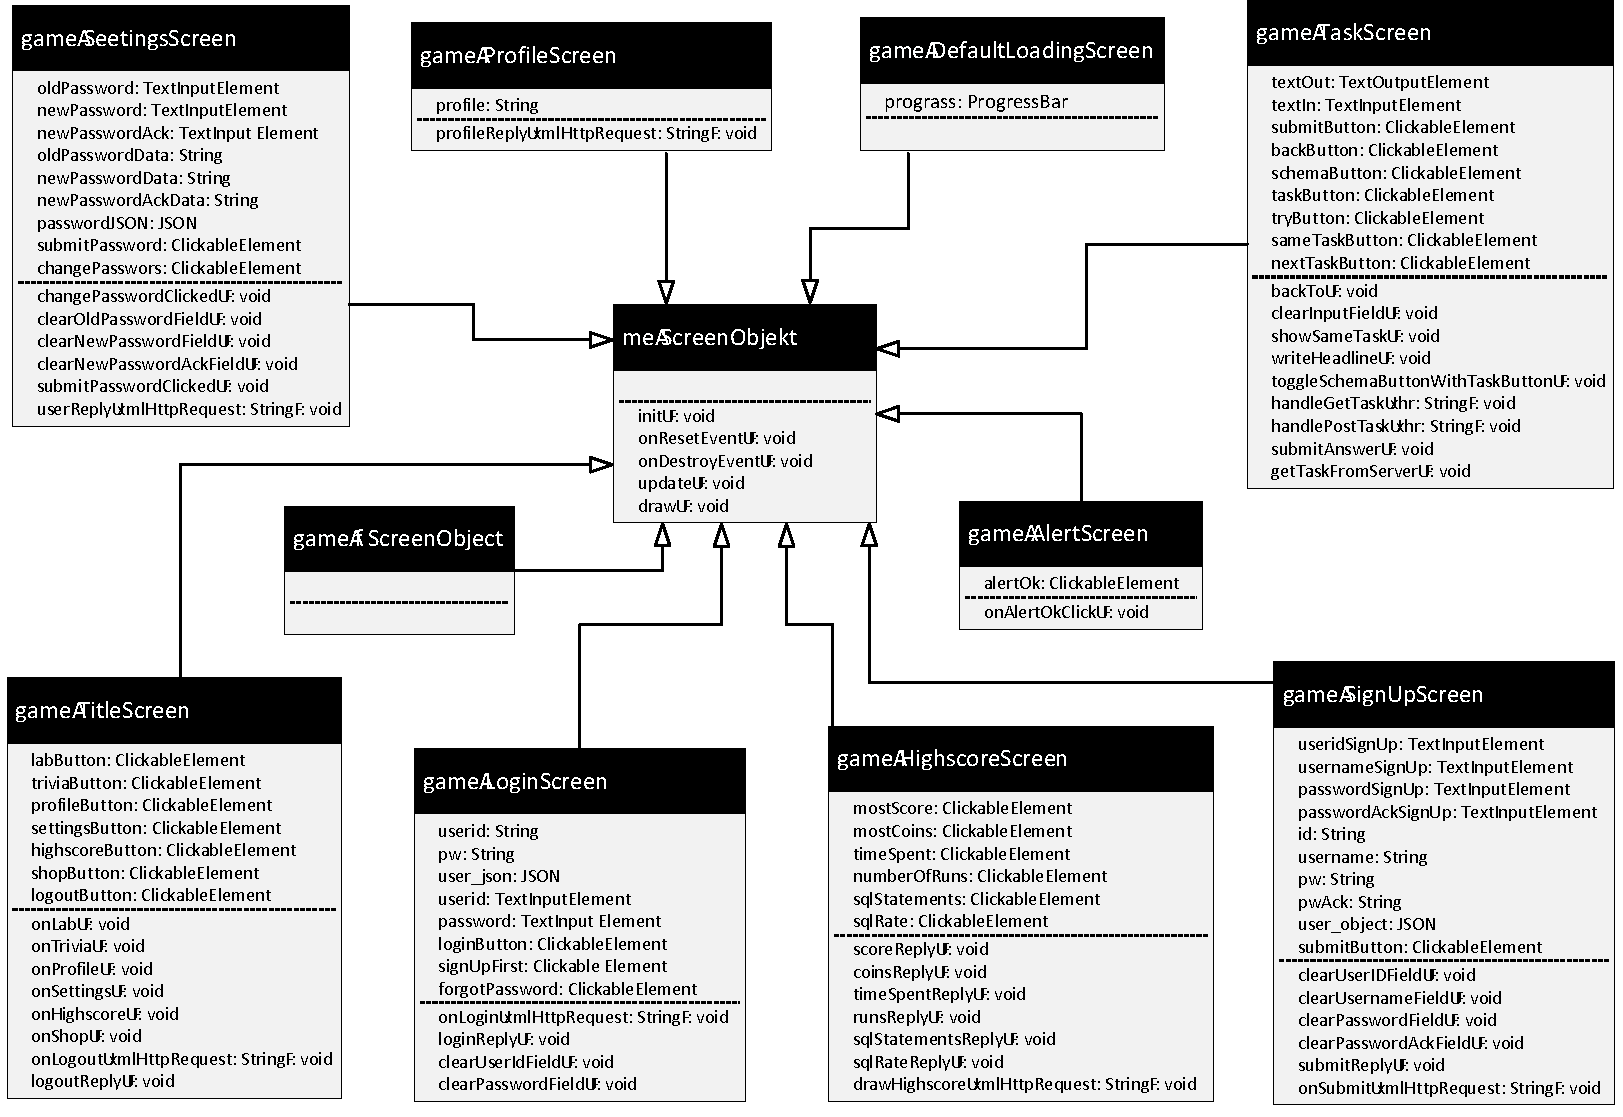
\includegraphics[width=1.0\textwidth]{figures/KLassendiagrammScreens.pdf}
\caption{Klassendiagramm für die verschiedenen Screens}
\label{MEscreen}
\end{figure}

\newpage
Des Weiteren gibt es folgende Screens mit zus\"atzlichen Funktionen.

\subsection{game.AlertScreen}
\label{Alert}
Der AlertScreen (STATE\_ALERT) wird aufgerufen, sobald der User mit einem Fehler konfrontiert werden muss. Gibt der User zum Beispiel falsche Eingaben beim
Login oder SignUp an, so wird er mittels dieses Screens darauf hingewiesen. Dazu besitzt er die Funktion OnAlertOkClick(). Wird der Alert zur Kenntnis 
genommen, schickt diese Funktion den Spieler in den letzten ausgew\"ahlten State und der automatische Reset dieses Screens wird ausgef\"uhrt.

\subsection{game.HighscoreScreen}
\label{Score}
Als motivationsf\"ordernden Faktor bietet die Applikation die M\"oglichkeit Ranglisten einzusehen. Diese befinden sich im HisghscoreScreen 
(Zustand: HIGHSCORE). Dieser Screen besitzt folgende Funktionen, die die jeweilige Highscore-Ajax-Anfrage an den Server abf\"angt:
 \begin{itemize}
	\item scoreReply();
	\item coinsReply();
	\item timeSpentReply();
	\item runsReply();
	\item sqlStatementsReply();
	\item sqlRateReply();
\end{itemize}
HINWEIS: Es handelt sich hierbei immer um GET-Anfragen, das hei{\ss}t, bei diesen Anfragen kommen immer Informationen zur\"uck ohne das neben der 
Anfrage selbst vorher Informationen an den Server mitgesendet werden m\"ussen.
Au{\ss}erdem gibt besitzt der game.HighscoreScreen noch eine drawHighscore(xmlHttpRequest)-Funktion die als Parameter das zuvor abgefangene 
Ergebnis der Ajax-Anfrage bekommt und dieses via der draw()-Funktion visualisiert.

\newpage
\subsection{game.DefaultLoadingScreen}
\label{Loading}
Der DefaultLoadingScreen ist ein visuell an das SQL-Alchemist-Thema angepasster Lade-Bildschirm. Dieser Screen besitzt das Element Progressbar 
und enthlt die Funktion progress(). progress() ist eine Funktion, \"ahnlich der update()-Funktion, mit dem prozentualen Fortschritt des Ladevorganges 
als Updatevariable, welche in game.js load() gestartet wird.

\subsection{game.LoginScreen}
\label{Login}
Dieser Screen (STATE\_LOGIN) bietet die Funktionalit\"at des Einloggens in die Applikation. Au{\ss}erdem wird dem Spieler hier die M\"oglichkeit gegeben 
durch einen entsprechenden Zustands-Wechsel in den STATE\_SIGNUP in den \nameref {SignUp} zu gelangen.
Die zus\"atzlichen Funktionen sind:
\begin{itemize}
	\item loginReply(): Diese Funktion f\"uhrt den Login aus. Sie ist daf\"ur zust\"andig die f\"ur den Login notwendigen Daten aus den
	         daf\"ur vorhandenen TextInputElemente (einfache Texteingabefelder) zu filtern, diese in ein JSON-Objekt zu parsen und per 
      		Ajax-POST-Anfgrage an den Server zu senden.
	\item onLogin(xmlHttpRequest): Die Funktion onLogin(xmlHttpRequest) bekommt als Parameter die Antwort der Ajax-Anfrage. Wenn 
	         dieser erfolgreich war \"andert die Funktion den STATE\_MENU und der\nameref {Title} wird geladen.
	\item clearUserIdField() und clearPasswordField(): Diese Funktionen dienen rein optischen Zwecken. Sie sorgen daf\"ur, dass der
      		 sogenannte Placeholder in den TextInputElements verschwindet und der User ungest\"ort seine Login-Daten eingeben kann. 
\end{itemize}

\subsection{game.SignUpScreen}
\label{SignUp}
Dieser Screen (STATE\_SIGNUP) bietet Funktionalit\"at des Registrierens f\"ur die Applikation. Nach Erfolg gelangt man in den TItleScreen. 
Daf\"ur notwendige Funktionen sind:
\begin{itemize}  
	\item submitReply() und onSubmit() sind f\"ur den SignUp \"aqiuvalente Funktionen zum \nameref {Login} .
 	\item clearUserIdField(), clearUserNameField(), clearPasswordField() und clearPasswordAckField() sind ebenfalls \"aquivalente Funktionen
	         zum L\"oschen der Placeholder. 
\end{itemize}  

\subsection{game.SettingsScreen}
\label{Settings}  
Der SeetingsScreen bietet dem User die M\"oglichkeit seine Spieleinstellungen zu \"andern. Der User kann Sound- und Musikeinstellungen \"andern und
au{\ss}erdem auch noch sein Passwort sowoh\"o zu \"andern, als auch es zur\"uckzusetzen. Um diese Funktionalit\"at zu gew\"ahrleisten fibt es folgende
Funktionen:
\begin{itemize}    
	\item changePasswordClicked(): Diese Funktion \"offnet drei Textfelder: oldPassword, newPassword und newPasswordAck. Diese sind f\"ur eine 
		 erfolgreiche Passwort\"anderung n\"otig.
	\item submitPasswordClicked(): Diese Funktion kontrolliert das neue Passw\"ort und dessen Best\"atigung. Sollten die \"ubereinstimmen wird userReply() 
		 aufgerufen.
	\item userReply(xmlHttpRequest): Diese Funktion sendet das neue Passwort per Ajax-Anfrage zum Server.
\end{itemize}    

\subsection{game.ProfileScreen}
\label{Profile}  
Im ProfileScreen werden dem User s\"amtliche Profilinformationen angezeigt. Daf\"ur existiert die Funktion profileReply(), die alle entsprechenden Daten
von dem Server bekommt. Dazu f\"uhrt diese Funktion eine Ajax-.Anfrage aus. Bei Erfolg werden die Profilinformationen mittels draw()-Funktion visualisiert.

\newpage
\subsection{game.TaskScreen}
\label{Task}  
Der TaskScreen repr\"asentiert in der Applikation den SQL-Trainer. f\"ur die Funktionalit\"at existieren folgende Funktionen:
\begin{itemize} 
	\item getTaskFromServer(): Diese Funktion sendet die Ajax-Anfrage an den Server und f\"uhrt im Anschluss writeHeadline() aus. Das Ergebnis der Anfrage wird
		an handleGetTask() als xhr Parameter \"ubergeben.
	\item handleGetTask(xhr): Diese Funktion f\"angt das Ergebnis der Anfrage ab. Dieses enth\"alt die zu l\"osende SQL-Aufgabe.
	\item writeHeadline(): Die Funktion schreibt die \"Uberschrift basierend auf die Aufgabe in den Screen.      
	\item toggleSchemaButtonWithTaskButton(): Mit Hilfe dieser Funktion kann der User zwischen der Anzeige des Aufgabentextes und des relationellen Schema 
		wechseln.
	\item submitAnswer(): Diese Funktion sendet die L\"osung des Users an den Server. Dies geschieht auch hier wieder \"uber eine Ajax-Anfrage.
	\item clearInputField(): Diese Funktion l\"oscht wie im \nameref {Login} beziehungsweise dem \nameref {SignUp} bereits erw\"ahnt den Placeholder des Texteingabefeldes.
\end{itemize}        

\subsection{game.TitleScreen}
\label{Title}  
Der TitleScreen beschreibt die Men\"uf\"uhrung der Applikation. Alle Buttons die einen durch einen Zustandswechsel in andere STATES und somit in andere Screens l
eitet, sind durch verschiedene Bilder dargestellt. Wichtige Funktionen die hier verwendet werden sind:
\begin{itemize} 
	\item logoutReply(): Diese Funktion sendet die Ajax-POST-Anfrage zum Logout an den Server. Bei Erfolg wird die beim Login erstellte User Session gel\"oscht.
	\item onLogout(xmlHttpRequest): Diese Funktion f\"angt das Ergebnis der Anfrage ab und der User wird den LoginScreen geleitet.
\end{itemize}    

\newpage
\subsection{me.GUI\_Object}
\label{GUI}
In den oben beschriebenen ScreenObjects befinden sich verschiedene Buttons. Die verwendeten Buttons stehen, wie in Abbildung \ref {MEgui} zu sehen is, mit einer EXTENDS-Beziehung
zu me.GUI\_Object in Verbindung. Alle Buttons erben von me.GUI\_Object die Funktion onClick() die ausgef\"uhrt wird, wenn der Button
geklickt wird. Alle Atrribute die an alle Buttons vererbt werden sind:
\begin{itemize} 
	\item settings.image: Diese Attribut enth\"alt den String mit dem Name des Bildes welches in den Hintergrund des Buttons geladen wird.
	\item settings.spriteheight : Dieses Attribut definiert die H\"ohe des Buttons.
  	\item settings.spritewidth: Dieses Attribut definiert dementsprechend die Breite des Buttons.
 	\item z: Der z-Index beschreibt die H\"ohe des Layers im Canvas. Niedrigere z-Indizes werden hierbei immer von gr\"o{\ss}eren \"uberschrieben.
\end{itemize}       
  
Folgende Buttons existieren in der Applikation und sind vollst\"andig durch die Extends-Beziehung definiert:
\begin{itemize} 
	\item task: Dieser Button \"ubergibt die Taskvariable difficulty und startet den STATE\_TASK.
	\item skinLeft: Dieser Button befindet sich im SheetScreen und geht die Liste an vorhandenen Avataren nach links ab.
	\item skinRight: Dieser Button ist der entsprechenden Button der die Liste der Avatare nach rechts durchgeht.
	\item potionArrow: Dieser Button wird durch einen kleinen Pfeil dargestellt, besitzt das Attribut currentPotion und ist in der Lage den ausgew\"ahlten Potion in 
		den ersten freien BeltSlot zu verschieben.
	\item beltSlotBelt: Dieser Button befindet sich im BeltScreen, besitzt ebenfalls das Attribut des zugeh\"origen Beltslot und hat besitzt die gegenteilige Funktion zum 
		potion Arrow. Der Button verschiebt den Inhalt des Beltslots in die PotionCollection.
	\item showPotion: showPotion befindet sich im BeltScreen. Die onClick()-Funktion auf den entsprechenden Potion \"ubergibt die  Taskvariblen (potionId und 
		difficulty) an den TaskScreen und startet diesen.
	\item next: next befindet sich im ResultScreen definiert eine einfache Weiterleitung in den TaskScreen.
	\item backToMenu: Dieser Button befindet sich in verschiedenen Screen. M\"ochte der User aus s\"amtlichen Screens zur\"uck in das Men\"u gelangen, so ist
		diese Funktionalit\"at durch diesen Button gegeben.
	\item backToLab: Dieser Button befindet sich ebenfalls auf verschiedenen Screens. durch einen Klick auf diesen, gelangt der User zur\"uck in das Laboratory.
\end{itemize}     

Au{\ss}erdem existieren Buttons in der Applikation die zus\"atzliche update()-Funktion besitzen. Diese Funktion f\"angt ein Event ab und agiert dementsprechend.
Die Events sind so definiert, dass sie durch Tastendruck aktiviert werden k\"onnen.
 
Diese Buttons sind:
\begin{itemize} 
  	\item exit: Dieser Button befindet sich im PlayScreen. Die zugewiesene Event-Taste ist die ESC-Taste. Diese beendet den Zustand PLAY und startet STATE\_GAMEOVER.
  	\item music: music befindet sich im PlayScreen mit dem Buchstaben M als EventTaste. Sie deaktiviert beziehungsweise reaktiviert die Hintergrundmusik des Minispiels.
	\item sound: sound befindet sich ebenfalls im PlayScreen und besitzt den Buchstaben N als EventTaste. Sie deaktiviert beziehungsweise reaktiviert die Soundeffekte des Minispiels.
  	\item beltSlot: Dieser Button befindet sich im PlayScreen. Es besitzt das Attribut n mit 1,2,3,...,n der den beltSlot des Uses definiert. Die EventTasten
	werden von Q bis R dem entsprechenden Slots zugewiesen, sodass der User die eingebundenen Potions im Spiel benutzen kann.
\end{itemize} 

\newpage
\begin{figure}[ht]
\centering
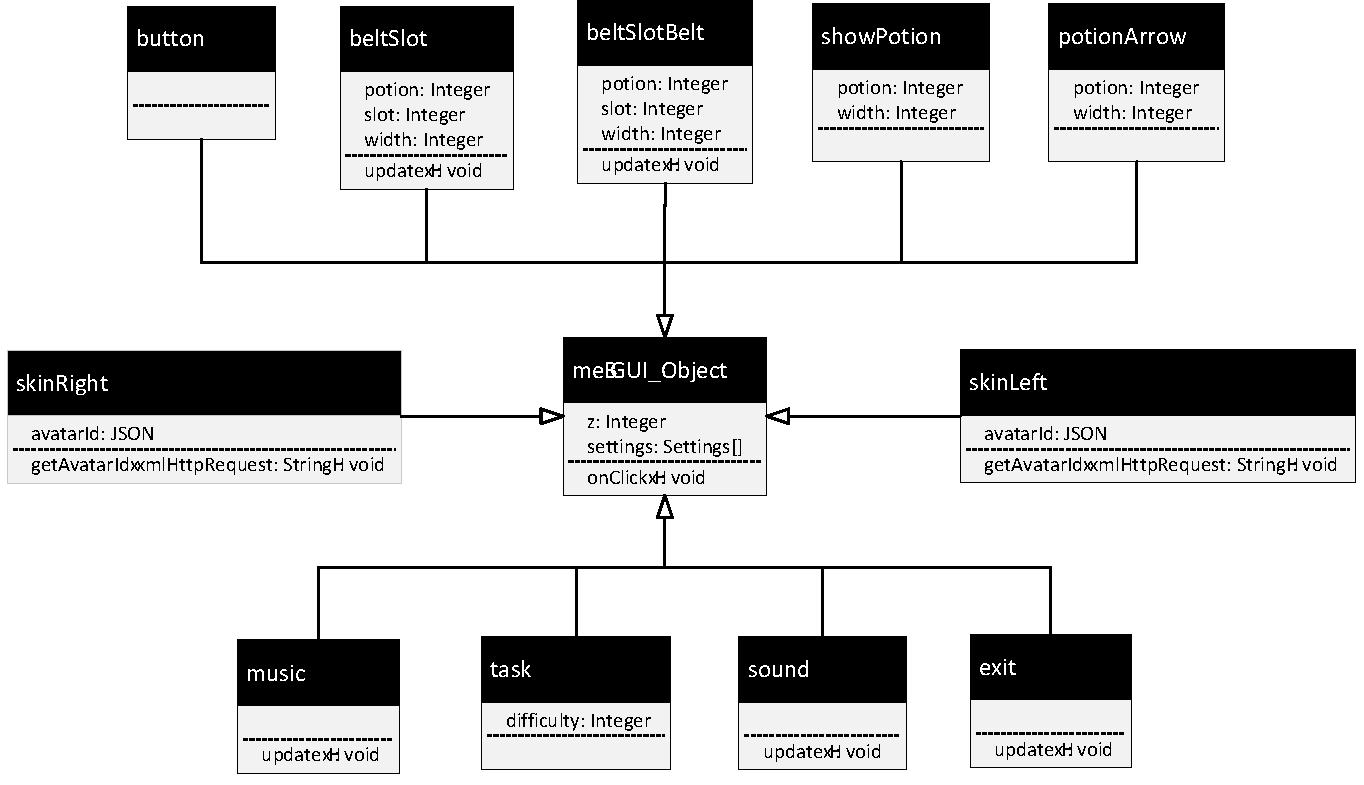
\includegraphics[width=1.0\textwidth]{figures/KlassendiagrammButtons.pdf}
\caption{Klassendiagramm für die verschiedenen Screens}
\label{MEgui}
\end{figure}    

\newpage
\subsection{me.Entity}
\label{Entity}
In dem Minispiel befinden sich diverse Entit\"aten. Diese stehen alle in einer EXTENDS-Beziehung mit me.Entity in Verbindung.
me.Entity besitzt folgende Variablen die an alle Entit\"aten vererbt werden:
\begin{itemize} 
	\item name: Die Variable name vom Typ String beschreibt den Namen der Entit\"at.
	\item body.collisionType: Dieses Attribut legt fest wie sich die Entit\"aten verhalten wenn sie kollidieren.
	\item body.velocity: Dieses Attribut besteht aus zwei Werten x und  y vom Typ Integer. Diese beschreiben die Bewegung der Entit\"at in horizontaler (x) 
		beziehungsweise vertikaler (y) Ebene.
 	\item alive: Die Variable alive vom Typ Boolean beschreibt, ob die Entity existiert. Der Default-Wert der Variable ist hierbei immer true.
\end{itemize}    

Au{\ss}erdem wird die Funktion init(), die dem Konstruktor in Java-Klassen entspricht, an die Entit\"aten vererbt. Sie definiert die Koordinaten und auf welcher Map
die Entit\"aten erzeugt werden.
  
Die einzelnen Entit\"aten im Minispiel sind folgende:

\newpage
\subsection{game.PlayerEntity}
\label{PlayerEntity}
Die PlayerEntity beschreibt die Spielfigur mit der der User durch das Dungeon l\"auft. Sie besitzt folgende zus\"atzliche Variablen und Funktionen:
\begin{itemize} 
 	\item alwaysUpdate: Diese Variable vom Typ Boolean wird abgefragt, wenn sich der Spieler au{\ss}erhalb des Viewports (Bildschirm) befindet. 
		Ist dieser Wert true, wird die update()-Funktion der Entity ausgef\"uhrt.
 	\item hurt: Dieses Attribut vom Typ  Boolean wird genau dann auf true gesetzt wenn der Spieler mit einem Gegner kollidiert. Um ein erneutes Aufrufen 
		der onCollision()-Funktion zu verhindern, wird nach einiger Zeit das hurt-Attribut auf false gesetzt.
 	\item settings.image: Diese Variable vom Typ String definiert den Namen des Bildes der Spielfigur.
  
 	\item update(dt): Die Funktion bekommt den Parameter dt \"ubergeben. Dies ist eine Zeitvariable, die definiert in welchen Abs\"anden die update-Funktion
		 ausgef\"uhrt werden soll. Sie aktualisiert die Position der Figur abh\"angig von der body.velocity und f\"angt das Jump-Event ab (wenn die Spielfigur 
		 zum Springen gebracht wurde). Au{\ss}erdem \"uberpr\"uft die Funktion ob die Hitbox der Spielfigur sich mit der einer anderen Entit\"at schneidet.               
                 Sie gibt true zur\"uck,  wenn die Verschiebung gerendert werden konnte.
               
 	\item onCollision(): Die Funktion analysiert wie und mit welcher Entit\"at die PlayerEntity kollidiert ist und reagiert dementsprechend. Sie gibt true zur\"uck, 
		wenn die PlayerEntity mit einem festen Element wie den B\"oden, den W\"anden und der Decke, kollidiert. Das Ergebnis ist false, wenn es 
		stattdessen eine andere Entit\"at war.
\end{itemize}    

\newpage
\subsection{game.LevelEntity}
\label{LevelEntity}
Die game.LevelEntity beschreibt das Wechseln der Level am Ende jeder Map. Kollidiert die PlayerEntity mit der LevelEntity so \"andert sich die Map.
Die zus\"atzlichen Variablen und Funktionen, die die LevelEntity besitzt, sind:
\begin{itemize} 
	\item goToLevel: Die Variable vom Typ String beschreibt den Namen der nach der Kollision zu ladenden Map.
	\item settings.to: Diese Variabel vom Typ Integer \"ubergibt die Schwierigkeit des n\"achsten Levels.
	\item settings.fade: Dieses Attribut vom Typ String beschreibt die Farbe des Fades in RGB-Werten.
	\item settings.duration: beschreibt die L\"ange des Fades in Millisekunden.

  	\item findNextLevel(): Die Funktion sucht zuf\"allig eine Map f\"ur das n\"achste Level eines gewissen Schwierigkeitsgrades aus. Sie gibt den Namen 
		der n\"achsten Map als String. Dieser Name wird in goToLevel gespeichert.
\end{itemize}    

\subsection{game.CoinEntity}
\label{CoinEntity}                               
game.CoinEntity, ist eine "Collectable Entity". Sie erh\"oht den Score des Users und wird beim Kollidieren mit der PlayerEntity gel\"oscht.
Die zus\"atzliche Funktion die nicht direkt von me.Entity geerbt wird, ist die onCollision()-Funktion. Sie wird durch das Kollidieren mit der PlayerEntity
 ausgel\"ost und erh\"oht den Score des Users.

\newpage
\subsection{game.SpikeEntity}
\label{SpikeEntity}                            
Die game.SpikeEntity ist ebenfalls eine "Collectable Entity". Die beendet den Lauf im Dungeon beim Kollidieren mit der PlayerEntity.
Auch diese Entit\"at besitzt die zus\"atzliche onCollision()-Funktion. Diese beendet den Lauf des Spielers und f\"uhrt einen Zustandswechsel in
den GAMEOVER-State

\subsection{game.ScrollEntity}
\label{ScrollEntity}    
Auch die game.ScrollEntity, ist eine "Collectable Entity". Der User sammelt diese ein und sie wird beim Kollidieren mit der PlayerEntity aus der Map entfernt.
Die zus\"atlichen Variablen und Funktionen sind:
\begin{itemize} 
	\item settings.scrollIndex: Diese Variable enth\"alt eine eindeutige ID der Scroll.
	\item settings.type: Diese Variable vom Typ String beschreibt den Typ der Scroll. Sie ist entweder eine  "Potion"-Scroll oder eine "Entchantent"-Scroll
	\item onCollision(): Diese Funktion wird durch das Kollidieren mit der PlayerEntity ausgel\"ost. Sie speichert die Scroll f\"ur den User und entfernt die Entity. 
\end{itemize}                      

\subsection{game.EnemyEntity}
\label{EnemyEntity}    
Die game.EnemyEntity beschreibt alle Gegner-Entit\"aten die im Minispiel vorkommen.
Die zus\"atzlichen Attribute und Funktionen die diese Entit\"aten besitzen sind:
\begin{itemize} 
	\item settings.spritewidth: Dieses Attribut vom Typ Integer beschreibt die Breite des Sprites der die Entit\"at im Spiel darstellt.
	\item settings.spriteheight: Dieses Attribut beschreibt entsprechend zur Breite des Sprites Die  H\"ohe.
	\item settings.jump: Das Attribut ist vom Typ Integer und definiert die Geschwindigkeit in vertikaler Ebene.
	\item settings.speed: Dieses Attribut beschreibt die Geschwindigkeit der Entit\"at in horizontaler Ebene.
	\item settings.attack: Integer: Diese Eigenschaft definiert die H\"ohe des Schadens den der Spieler bekommt, wenn er mit der EnemyEntity kollidiert.
	\item startY: Dieses Attribut vom Typ Integer entspricht der y-Koordinate von me.Entity bei der Initiallisierung.
	\item startX: Dieses Attribut vom Typ Integer entspricht dementsprechend der x-Koordinate von me.Entity.
	\item pos.Y: In dieser Variable wird die aktuelle y-Koordinate der Entit\"at gespeichert.
	\item pos.X: In dieser Variable wird dementsprechend die x-Koordinate der Entit\"at gespeichert.
	\item endY: endY vom Typ Integer beschreibt die y-Koordinate, welche das Ende des Bereiches, in welchem sich die Gegner-Entit\"at bewegen darf.
	\item endX: endX ist entsprechend zu endY die x-Koordinate des Bereichs in der sich die Entit\"at bewegen darf.
	\item jump: Dieses Attribut vom Typ Boolean wird genau dann auf true gesetzt, wenn die Gegner-Entit\"at spring beziehungsweise fliegt und false wenn 
		sie f\"allt. Der Default-Wert dieser Variable ist false gesetzt.
	\item walkLeft: Dieses Attribut vom Typ Boolean wird auf Ist true gesetzt, wenn sich die Gegner-Entit\"at nach links bewegt und false wenn sie 
		nach rechts geht. Auch dieses Attribut ist stndartm\"a{\ss}ig auf false gesetzt. 
	\item update(): Diese Funktion l\"ast die EnemyEntity nach links laufen und fliegen. Erreicht die Entit\"at endY oder endX kehrt sie um l\"auft nach 
		rechts und f\"allt bis zu startY und startX. Die Funktion gibt true zur\"uck wenn das Rendern der Entit\"at auf der neuen Position erfolgreich war.
	\item body.setVelocity(): Diese Funktion legt horizontale und vertikale Bewegungen fest.
\end{itemize}  


\newpage
\begin{figure}[ht]
\centering
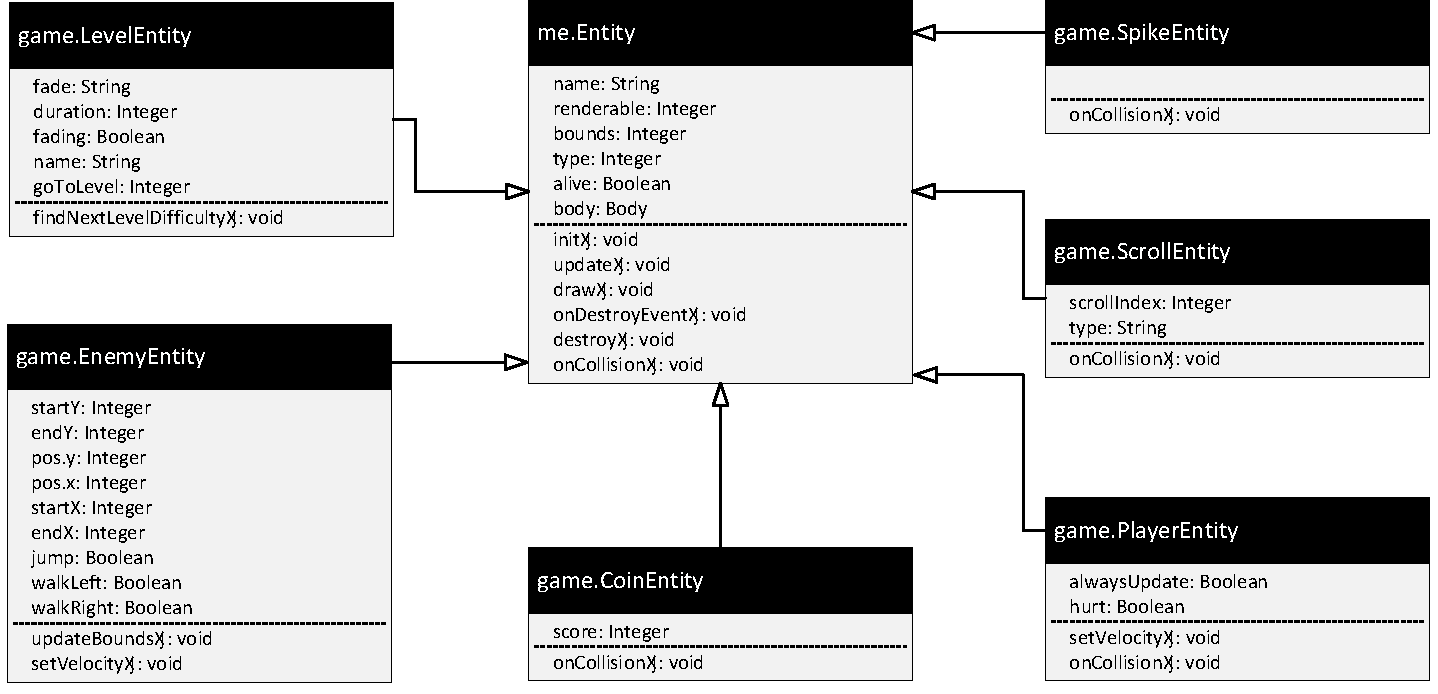
\includegraphics[width=1.0\textwidth]{figures/KlassendiagrammFrontEndEntities.pdf}
\caption{Klassendiagramm für die verschiedenen Front-End-Entitäten}
\label{MEentity}
\end{figure}   

\newpage    

% HERE BEGIN


%\subsection{game.me.Container}
%Container sind da um verschiedene HUDs und buttons zu b¸ndeln und ihnen gemeinsame Eigenschaften zu geben. Die Eigenschaften der HUDs
%und buttons werden an deren Stellen genauer beschrieben.
%Sie besitzen folgende Variablen:
 % - isPersistent: Boolean: Wenn true kann der Contaier nicht ver‰ndert werden.
 % - floating: Boolean: Wenn true bewegen sich die Elemente des Containers mit dem Viewport(Spierler Bildschirm) mit.
 % - name: String: Name des Containers.
%  - z: Integer: Beschreibt die Hˆhe in welcher Element des Containers in den Canvas geladen werden.
%und die Konstruktorfunktion:
 % - init(): Entspricht dem Konstruktor in Java.
  
%In der Applikation befinden sich 2 Container alle extenden von me.Container deren.
%Die Container werden im Minispiel eingeladen.
 
%- game.HUD.Container
%In den Container werden folgende HUDs eingetragen
 % - HUD.ScoreItem
  %- HUD.HealthScore

% - game.HUDII.Container
%In den Container werden folgende Buttons eingetragen
% - beltSlots
% - sound
% - music
% - exit
 
%me.Sprite
%Bilder die ohne jegliche besondere Eigenschaften eingeladen werden.
%Sie besitzen folgende Variablen:
%  - z: Integer: Beschreibt die Hˆhe in welcher Element des Containers in den Canvas geladen werden.
%und die Konstruktorfunktion:
%  - init(): Entspricht dem Konstruktor in Java.
  
%game.Icon extendet von me.Sprite

%game.SkinFront
%besitzt folgende Variablen:
%  - currentSkin: String: Name des Skins. Wird als Updatevariable benutzt.
%und folgende Funktion:
%  - update(dt): Der Parameter: dt ist die Zeitvariable in welchen Abst‰nden update ausgef¸hrt wird.
%                L‰dt das Bild neu wenn es ge‰ndert wird.


%END HERE      
          
\subsection{me.Renderable}
\label{Render}                   
Alle HUDs (Head-Up-Displays) stehen in einer EXTENDS-Beziehung zu me.Renderable. HUDs werden in derApplikation daf\"ur verwendet, Texte zu 
in die Screens zu schreiben und diese zur Laufzeit zu aktualisieren.
Sie besitzen folgende Variablen und Funktionen:
\begin{itemize} 
	\item font: Das font-Attribut enth\"alt dem Schrifttyp der in der draw()-Funktion benutzt wird.
	\item init(): Diese Funktion entspricht dem Konstruktor in Java und initialisiert das HUD.
	\item update(): Diese Funktion aktualisiert das HUD. Sie gibt true zur\"uck, wenn der eingef\"ugte Text erfolgreich gerendert werden konnte.
	\item draw(): Diese Funktion enth\"alt den Text der auf das HUD geschrieben werden soll.
\end{itemize}                     

Alle HUDs die von me.Renderable erben sind:
\begin{itemize} 
	\item game.HUD.ScoreItem: Dieses HUD schreibt den Score des Spielers das im Minispiel angezeigt wird.
	\item game.HUD.HealthScore: Dieses HUD schreibt die Leben die der User aktuell im Minispiel besitzt.
	\item game.HUD.SkinName: Dieses HUD schreibt den Namen des entsprechenden, ausgew\"ahlten Avatares. Es wird im SheetScreen verwendet.
	\item game.HUD.SettingsElements: Dieses HUD schreibt die Einstellungen des User in den \nameref {Settings}.
	\item game.HUD.GameOver: Dieses HUD schreibt alle Informationen des GameOverScreens.
	\item game.HUD.Result: Dieses HUD schreibt den Inhalt des ResultScreens.
	\item game.HUD.Profile: Der Inhalt des \nameref {Profile} werden in diesem HUD geschrieben.
	\item game.HUD.PotionAmount: Dieses HUD schreibt die Anzahl der vorhanden Potions in den BeltScreen.
	\item game.HUD.Shop: Dieses HUD schreibt die Anzahl der Lofi-Coins in den ShopScreen.
	\item game.HUD.OverlayAlert: Dieses HUD schreibt die Fehlermeldungen in den AlertScreen.
\end{itemize} 

\newpage
\begin{figure}[ht]
\centering
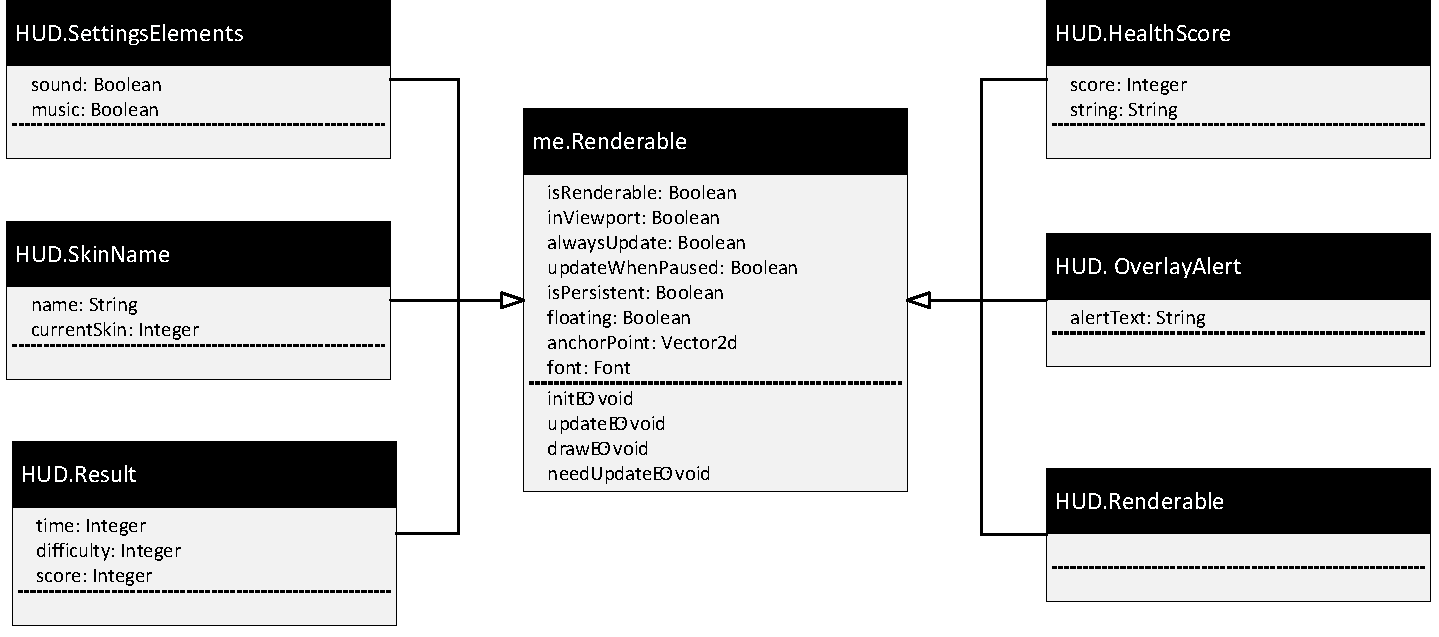
\includegraphics[width=1.0\textwidth]{figures/KLassendiagrammRenderables.pdf}
\caption{Klassendiagramm für die Renderables}
\label{MErenderable}
\end{figure}    

\newpage


\newpage
\section{Implementierung von Komponente <C20>: Das Back-End}
\label{backend}

Im folgenden Abschnitt soll detaillierter auf die Implementierung der Back-End-Komponente eingegangen werden.

Das Back-End des SQL-Alchemist hat die Aufgabe, die spielinterne Datenbank zu verwalten. Dabei müssen die anfallenden Daten korrekt gespeichert und dem Front-End auf Anfrage zur Verfügung gestellt werden.

Bei der Entwicklung dieser Komponente wird auf zwei Bibliotheken zurückgegriffen. Zunächst gehört dazu das play!-Framework, welches dazu dient webbasierte Anwendungen zu erstellen. Dabei stellt es zusätzlich auch die im Projekt verwendete Datenbank zur Verfügung. Die zweite verwendete Bibliothek wird vom Teamprojekt entwickelt und prüft SQL-Statements auf ihre Korrektheit. Dies wird beim SQL-Modul des SQL-Alchemisten Anwendung finden. 

Im ersten Unterkapitel wird die Komponente durch Klassendiagramme dargestellt. Der Übersicht halber wurden die Klassen dabei auf mehrere Diagramme verteilt, da der Umfang der Komponente den Rahmen einer Seite übersteigen würde. Um den Zusammenhang der einzelnen Diagramme untereinander zu verdeutlichen werden Klassen, die Assoziationen zu Klassen in anderen Diagrammen haben, in diesen ebenfalls, aber ohne Attribute und Methoden, dargestellt.  

Im zweiten Unterkapitel werden dann jeweils noch kurz die einzelnen Klassen, sowie deren Attribute und Methoden beschrieben.

\clearpage


\newpage


\subsection{Model Classes -- Profile}
\subsection{Paket-/Klassendiagramm}
\begin{figure}[h!]
\centering
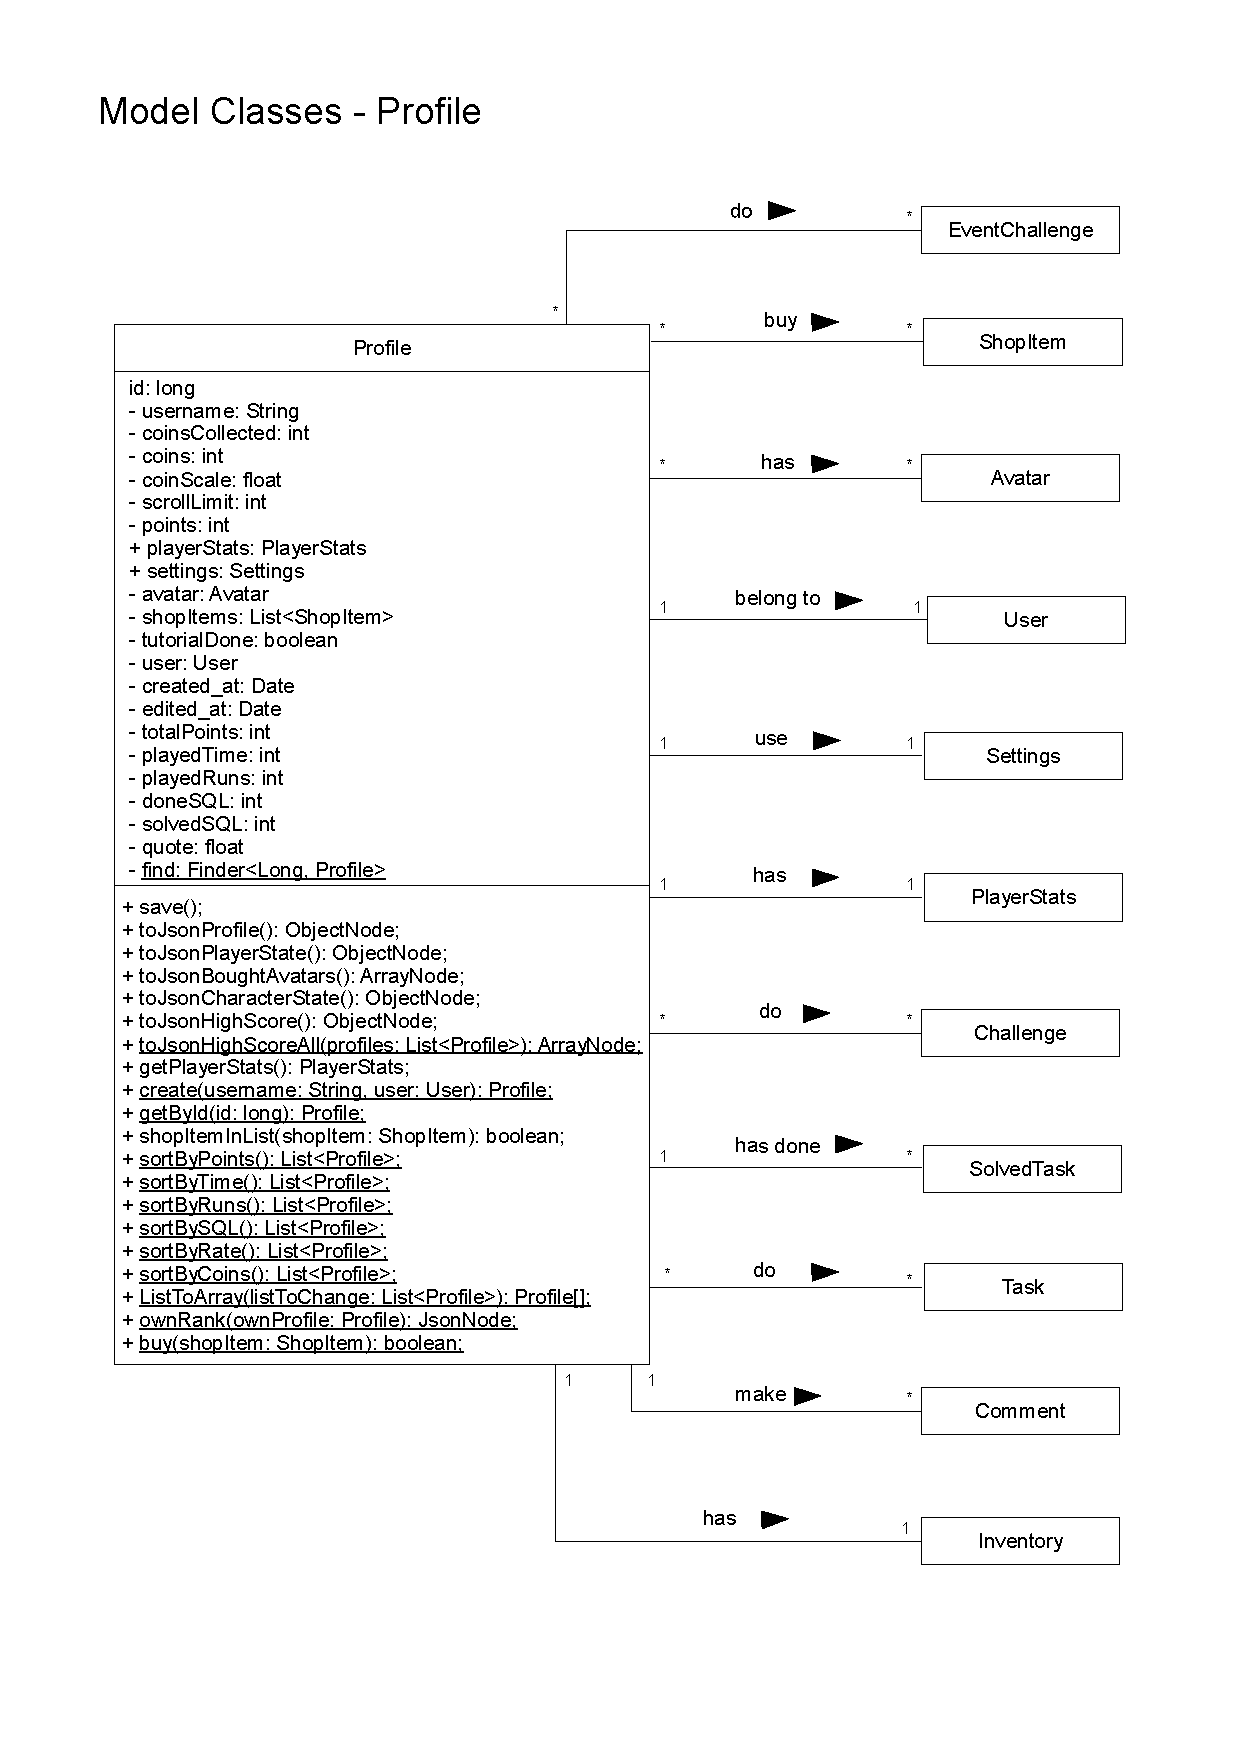
\includegraphics[width=0.8\textwidth]{figures/KDProfile}
\caption{Klassendiagramm für die Model-Klasse Profile \ref{C20}}
\label{classC10}
\end{figure}
\clearpage
\subsection{Erläuterung}
\begin{class}{10}{Profile}
\item[Aufgabe]~\\
Verwaltung der Nutzerprofile des SQL-Alchemist
\item[Attribute]~\\
\begin{itemize}
\item id:long -- Einzigartige ID
\item username: String -- Benutzername des zugehörigen Nutzers
\item coinsCollected: int -- Anzahl der bisher gesammelten Lofi-Coins
\item coins: int -- Anzahl der momentanen Lofi-Coins des Nutzers
\item coinScale: float -- 
\item scrollLimit: int -- Anzahl der maximal sammelbaren Schriftrollen pro Zeitraum
\item points: int -- Die Punkte des Spielers
\item playerStats: PlayerStats -- Die Attribute der Spielfigur des Nutzers
\item settings: Settings -- Die vom Nutzer gewählten Einstellungen
\item avatar: Avatar -- Der vom Nutzer gewählte Avatar
\item shopItems: List<ShopItem> -- Bisher vom Nutzer gekaufte Gegenstände
\item tutorialDone: boolean -- Hält fest ob das Tutorial bereits vom Nutzer bearbeitet wurde
\item user: User -- Der zum Profil gehörige Nutzer
\item created\_at: Date -- Zeitpunkt zu dem das Profil erstellt wurde
\item edited\_at: Date -- Zeitpunkt zu dem das Profil zuletzt bearbeitet wurde
\item totalPoints: int -- Gesamtzahl der vom Nutzer erspielten Punkte
\item playedTime: int -- Bisher im Spiel verbrachte Zeit
\item playedRuns: int -- Bisher gespielte Durchläufe
\item doneSQL: int -- Bisher bearbeitete SQL-Aufgaben
\item solvedSQL: int -- Bisher korrekt gelöste SQL-Aufgaben
\item quote: float -- Rate von gelösten SQL-Aufgaben im Vergleich zu bearbeiteten Aufgaben
\item find: Finder<Long, Profile> -- Der Finder der Klasse zum Suchen in der Datenbank
\end{itemize}
\item[Operationen]~\\
\begin{itemize}
\item save() -- Diese Methode speichert das Profil
\item toJsonProfile(): ObjectNode -- Erzeugt aus einem Profildatensatz ein Json-Objekt
\item toJsonPlayerState(): ObjectNode -- Erzeugt aus einem Profildatensatz ein auf den PlayerState spezialisiertes Json-Objekt
\item toJsonBoughtAvatars(): ArrayNode -- Erzeugt ein Json-Array in welchem die gekauften Avatare gespeichert sind
\item toJsonCharacterState(): ObjectNode --
Erzeugt aus einem Profildatensatz ein auf den CharacterState spezialisiertes Json-Objekt
\item toJsonHighScore(): ObjectNode -- Erzeugt aus einem Profildatensatz ein für die Ranglisten spezialisiertes Json-Objekt
\item toJsonHighScoreAll(profiles: List<Profile>): ArrayNode -- Erstellt ein für die Ranglisten spezialisiertes Json-Array, welches mehrere Profileinträge enthält
\item getPlayerStats(): PlayerStats -- Kombiniert die PlayerStats des Avatars mit denen des Nutzers und gibt diese zurück
\item create(username: String, user: User): Profile -- Erstellt einen neuen Profildatensatz
\item getById(id: long): Profile -- Sucht ein Profil anhand dessen ID und gibt es zurück
\item shopItemInList(shopItem): boolean -- Prüft, ob ein ShopItem bereits gekauft wurde
\item sortByPoints(): List<Profile> -- Gibt eine Liste der, nach Punkten sortiert, zehn besten Profile zurück
\item sortByTime(): List<Profile> -- Gibt eine Liste der, nach Spielzeit sortiert, zehn besten Profile zurück
\item sortByRuns(): List<Profile> -- Gibt eine Liste der, nach Durchläufen sortiert, zehn besten Profile zurück
\item sortBySQL(): List<Profile> -- Gibt eine Liste der, nach gelösten SQL-Aufgaben sortiert, zehn besten Profile zurück
\item sortByRate(): List<Profile> -- Gibt eine Liste der, nach Erfolgsquote sortiert, zehn besten Profile zurück
\item sortByCoins(): List<Profile> -- Gibt eine Liste der, nach gesammelten Lofi-Coins sortiert, zehn besten Profile zurück
\item ListToArray(listToChange: List<Profile>): Profile[] -- Erzeugt ein Array aus einer Liste
\item ownRank(ownProfile: Profile): JsonNode -- Erzeugt ein für die Ranglisten spezialisiertes Json-Objekt
\item buy(shopItem: ShopItem): boolean -- Prüft, ob der Nutzer genügend Coins hat um ein ShopItem zu kaufen und führt dann den Kauf durch
\end{itemize}
\item[Kommunikationspartner]~\\
\begin{itemize}
\item EventChallenge
\item ShopItem
\item Avatar
\item User
\item Settings
\item PlayerStats
\item Challenge
\item SolvedTask
\item Task
\item Comment
\item Inventory
\end{itemize}
\end{class}

\newpage
\subsection{Model Classes -- Part 1}
\subsection{Paket-/Klassendiagramm}
\begin{figure}[h!]
\centering
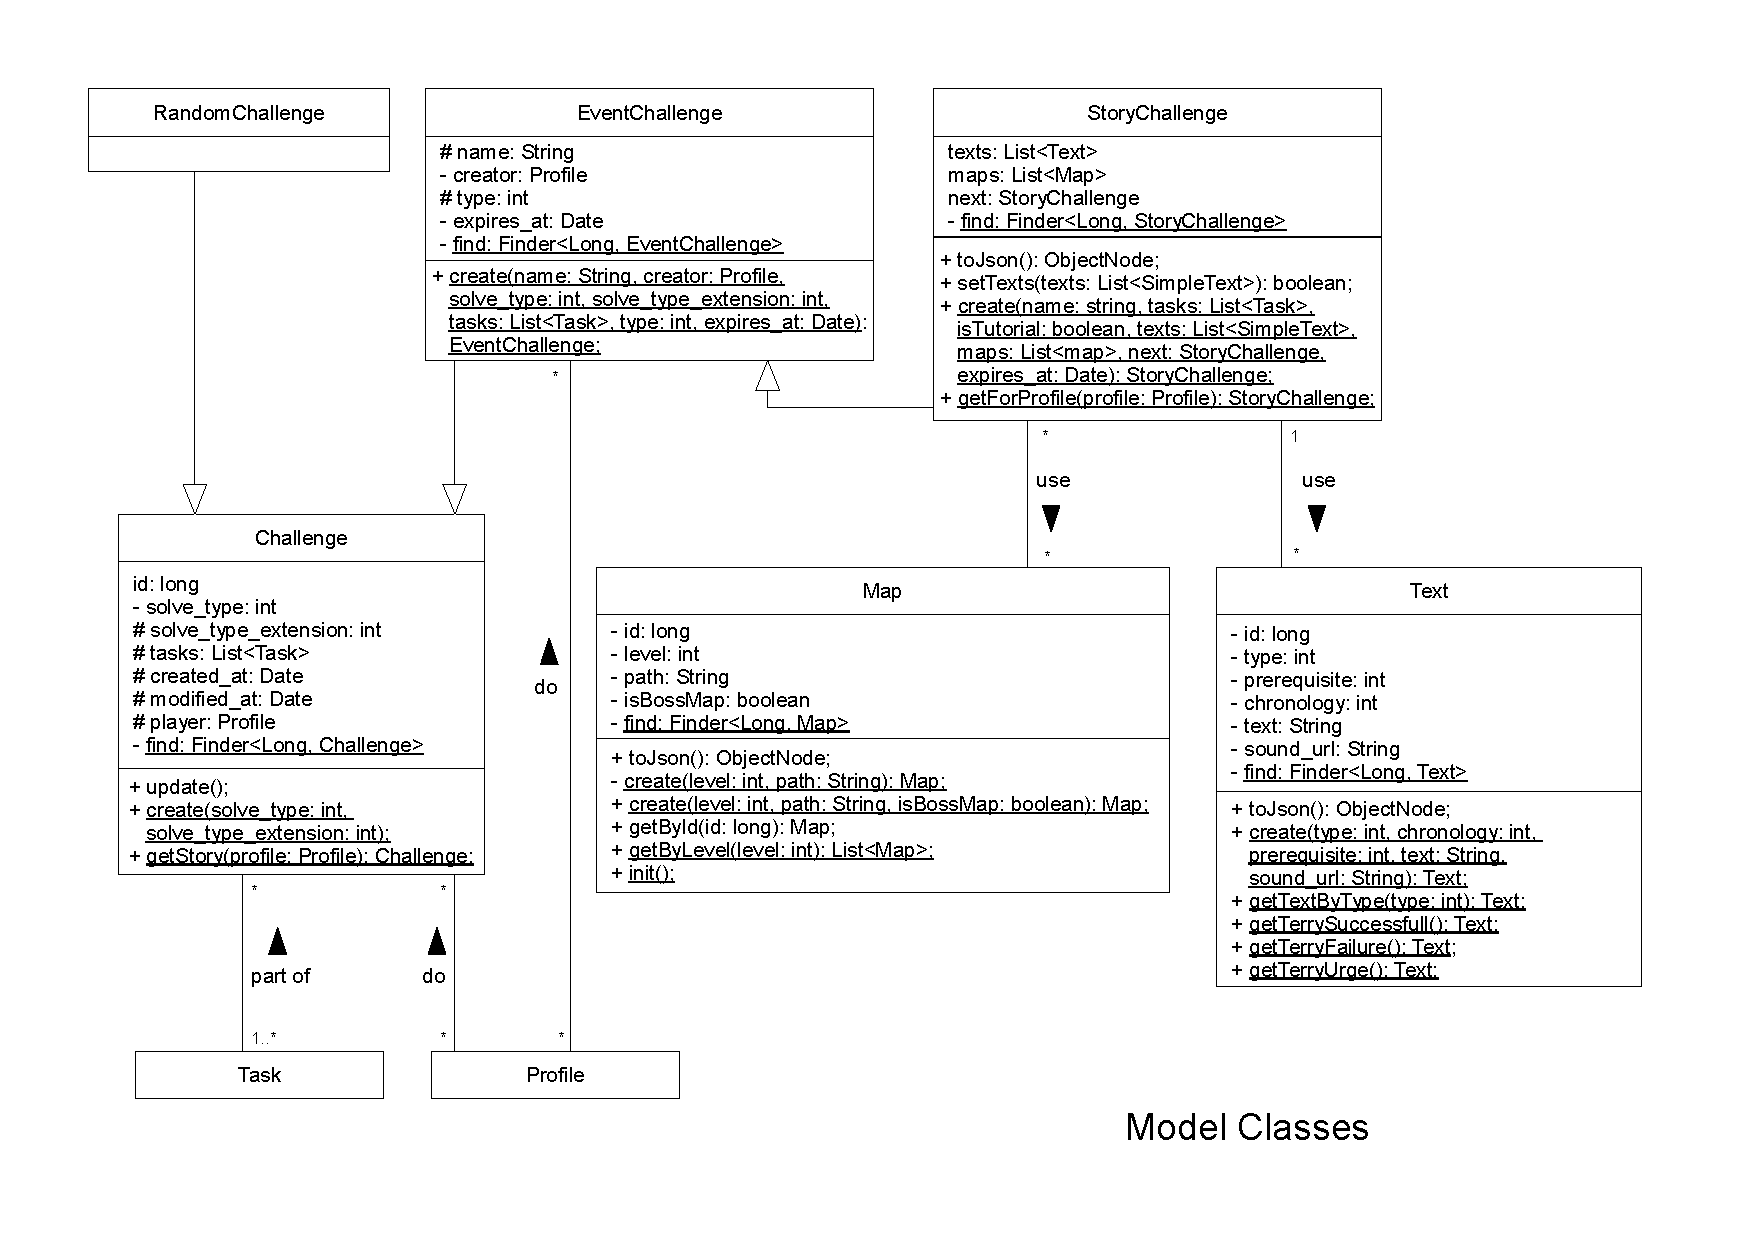
\includegraphics[width=0.8\textwidth]{figures/KDChallenge}
\caption{Klassendiagramm für einige der Model-Klassen \ref{C20}}
\label{classC10}
\end{figure}
\clearpage
\subsection{Erläuterung}
\begin{class}{20}{Challenge}
\item[Aufgabe]~\\
Verwaltung der Aufgabenpakete
\item[Attribute]~\\
\begin{itemize}
\item id: long -- Einzigartige ID
\item solve\_type: int -- Beschreibt die Eigenschaften des Paketes hinsichtlich dessen Lösung
\item solve\_type\_extension: int -- Zusatz zu den Eigenschaften des Aufgabenpaketes
\item tasks: List<Task> -- Eine Liste der im Paket enthaltenen Aufgaben
\item created\_at: Date -- Zeitpunkt zu dem das Aufgabenpaket erstellt wurde
\item modified\_at: Date -- Zeitpunkt zu dem das Aufgabenpaket zuletzt geändert wurde
\item player: Profile -- Spieler, denen das Aufgabenpaket gestellt wird
\item find: Finder<Long, Challenge> -- Der Finder der Klasse zum Suchen in der Datenbank
\end{itemize}
\item[Operationen]~\\
\begin{itemize}
\item update() -- Aktualisiert das Aufgabenpaket
\item create(solve\_type: int, solve\_type\_extension: int) -- Erstellt ein neues Aufgabenpaket
\item getStory(profile: Profile): Challenge -- Gibt die Story zurück
\end{itemize}
\item[Kommunikationspartner]~\\
\begin{itemize}
\item Task
\item Profile
\item RandomChallenge
\item EventChallenge
\end{itemize}
\end{class}

\newpage
\begin{class}{30}{RandomChallenge}
\item[Aufgabe]~\\
Verwaltet das zufällige Stellen von Aufgabenpaketen
\item[Attribute]~\\
Keine
\item[Operationen]~\\
Keine
\item[Kommunikationspartner]~\\
\begin{itemize}
\item Challenge
\end{itemize}
\end{class}

\newpage
\begin{class}{40}{EventChallenge}
\item[Aufgabe]~\\
Verwaltung der Aufgabenpakete für spezielle Events
\item[Attribute]~\\
\begin{itemize}
\item name: String -- Name des Aufgabenpaketes
\item creator: Profile -- Der Nutzer, der das Paket erstellt hat
\item type: int -- Der Typ des Paketes
\item expires\_at: Date der Zeitpunkt, wann das Aufgabenpaket nicht mehr gelöst werden kann
\item find: Finder<Long, EventChallenge> -- Der Finder der Klasse zum Suchen in der Datenbank
\end{itemize}
\item[Operationen]~\\
\begin{itemize}
\item create(name: String, creator: Profile, solve\_type: int, solve\_type\_extension: int, tasks: List<Task>, type: int, expires\_at: Date): EventChallenge -- Erstellt ein neues Aufgabenpaket
\end{itemize}
\item[Kommunikationspartner]~\\
\begin{itemize}
\item Profile
\item Challenge
\item StoryChallenge
\end{itemize}
\end{class}

\newpage
\begin{class}{50}{StoryChallenge}
\item[Aufgabe]~\\
Verwaltung der Aufgabenpakete für den Story-Modus
\item[Attribute]~\\
\begin{itemize}
\item texts: List<Text> -- Eine Liste der im Aufgabenpaket verwendeten Texte
\item maps: List<Map> -- Eine Liste der im Aufgabenpaket verwendeten Karten
\item next: StoryChallenge -- Das Aufgabenpaket, welches auf das aktuelle folgt
\item find: Finder<Long, StoryChallenge> -- Der Finder der Klasse zum Suchen in der Datenbank
\end{itemize}
\item[Operationen]~\\
\begin{itemize}
\item toJson(): ObjectNode -- Erstellt aus dem Paket ein Json-Objekt
\item setTexts(texts: List<SimpleText>): boolean -- Fügt dem Paket neue Texte hinzu
\item create(name: String, tasks: List<Task>, isTutorial: boolean, texts: List<SimpleText>, maps: List<map>, next: StoryChallenge, expires\_at: Date): StoryChallenge -- Erstellt ein neues Aufgabenpaket
\item getForProfile(profile: Profile): StoryChallenge -- Weist das Aufgabenpaket einem Profil zu
\end{itemize}
\item[Kommunikationspartner]~\\
\begin{itemize}
\item Map
\item Text
\item EventChallenge
\end{itemize}
\end{class}

\newpage
\begin{class}{60}{Map}
\item[Aufgabe]~\\
Verwaltung der Minispiel-Karten
\item[Attribute]~\\
\begin{itemize}
\item id: long -- Einzigartige ID
\item level: int -- Gibt den Level dar, in dem die Karte verwendet wird
\item path: String -- Der Pfad an dem die Karte abgespeichert ist
\item isBossMap: boolean -- Legt fest, ob die Karte eine Karte mit Endgegner ist
\item find: Finder<Long, Map> -- Der Finder der Klasse zum Suchen in der Datenbank
\end{itemize}
\item[Operationen]~\\
\begin{itemize}
\item toJson(): ObjectNode -- Erstellt aus dem Kartendatensatz ein Json-Objekt
\item create(level: int, path: String): Map -- Erstellt einen neuen Kartendatensatz
\item create(level: int, path: String, isBossMap: boolean): Map -- Erstellt einen neuen Kartendatensatz
\item getById(id: long): Map -- Sucht eine Karte anhand ihrer ID
\item getByLevel(level: int): List<Map> -- Sucht alle Karten, die in einem bestimmten Level vorkommen
\item init() -- Initialisiert die Karten
\end{itemize}
\item[Kommunikationspartner]~\\
\begin{itemize}
\item StoryChallenge
\end{itemize}
\end{class}

\newpage
\begin{class}{70}{Text}
\item[Aufgabe]~\\
Verwaltung der Texte für den Story-Modus
\item[Attribute]~\\
\begin{itemize}
\item id: long -- Einzigartige ID
\item type: int -- Art des Textes
\item prerequisite: int -- Bedingung, die erfüllt sein muss, damit der Text aufgerufen wird
\item chronology: int -- Reihenfolge, in der die Texte auftreten
\item text: String -- Der eigentliche Text
\item sound\_url: String -- Der zum Text gehörende Sound
\item find: Finder<Long, Text> -- Der Finder der Klasse zum Suchen in der Datenbank
\end{itemize}
\item[Operationen]~\\
\begin{itemize}
\item toJson(): ObjectNode -- Erzeugt aus dem Textdatensatz ein Json-Objekt
\item create(type: int, chronology: int, prerequisite: int, text: String, sound\_url: String): Text -- Erstellt einen neuen Textdatensatz
\item getTextByType(type: int): Text -- Sucht einen zufälligen Text eines bestimmten Typs heraus und gibt ihn zurück
\item getTerrySuccessfull(): Text -- Sucht einen Text mit positiven Kommentar von Terry zurück
\item getTerryFailure(): Text -- Sucht einen Text mit negativen Kommentar von Terry zurück
\item getTerryUrge(): Text -- Sucht einen Text mit drängendem Kommentar von Terry zurück
\end{itemize}
\item[Kommunikationspartner]~\\
\begin{itemize}
\item StoryChallenge
\end{itemize}
\end{class}

\newpage
\subsection{Model Classes -- Part 2}
\subsection{Paket-/Klassendiagramm}
\begin{figure}[h!]
\centering
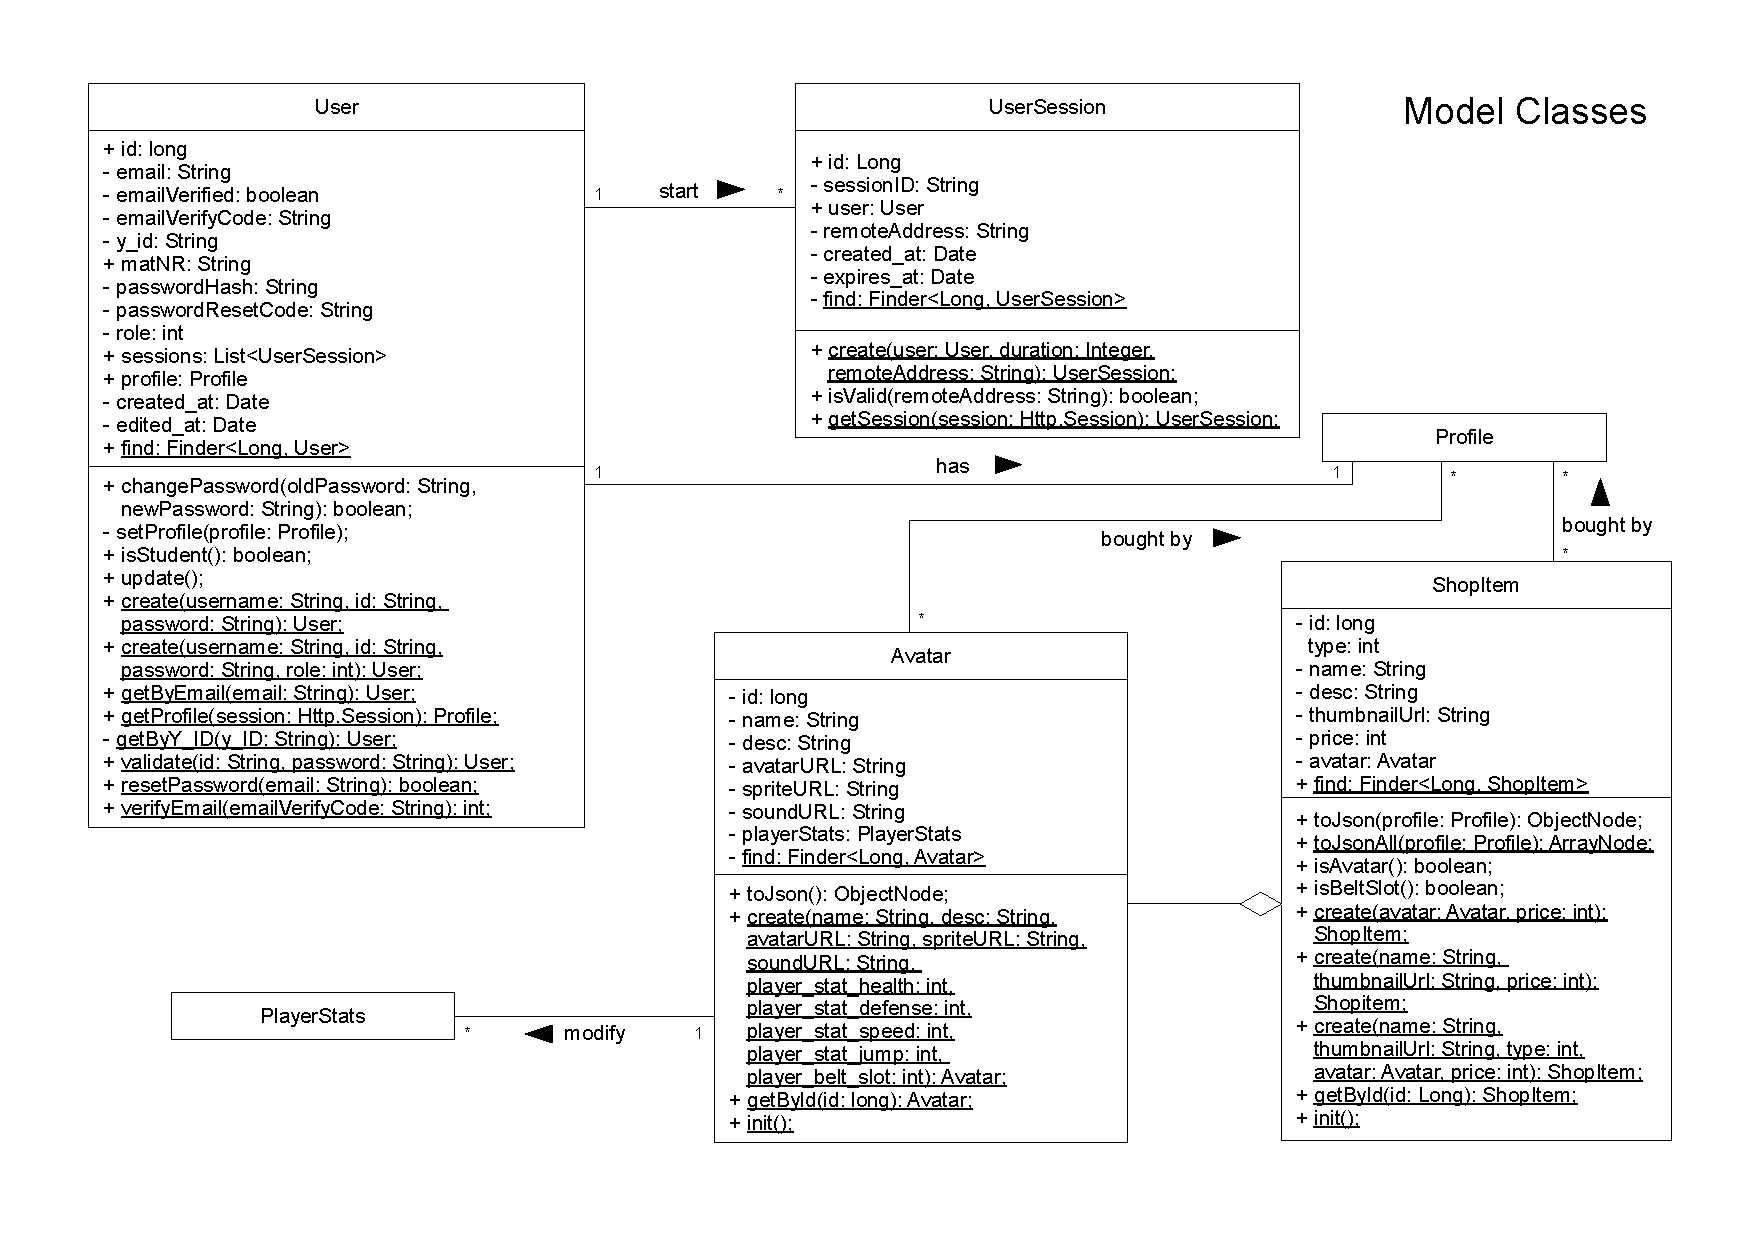
\includegraphics[width=0.8\textwidth]{figures/KDUserAndAvatar}
\caption{Klassendiagramm für einige der Model-Klassen \ref{C20}}
\label{classC10}
\end{figure}
\clearpage
\subsection{Erläuterung}
\begin{class}{80}{User}
\item[Aufgabe]~\\
Verwaltung der Nutzer
\item[Attribute]~\\
\begin{itemize}
\item id: long -- Einzigartige ID
\item email: String -- Email-Adresse des Nutzers
\item emailVerified: boolean -- Legt fest, ob die Adresse bereits verifiziert ist
\item emailVerifyCode: String -- Der Verifizierungscode der Adresse
\item y\_id: String -- Die y-Nummer des Nutzers (falls der Nutzer ein Student ist)
\item matNR: String -- Die Matrikelnummer des Nutzers (falls der Nutzer ein Student ist)
\item passwordHash: String -- Der Passwort-Hash des Nutzers
\item passwordResetCode: String -- Der Code zum Zurücksetzen des Passworts
\item role: int -- Rechtegruppe, welcher der Nutzer angehört
\item sessions: List<UserSession> -- Liste an Sitzungen, die der Nutzer gestartet hat
\item profile: Profile -- Das Profil des Nutzers
\item created\_at: Date -- Zeitpunkt zu dem sich der Nutzer registriert hat
\item edited\_at: Date -- Zeitpunkt zu dem zuletzt etwas am Nutzerdatensatz geändert wurde
\item find: Finder<Long, User> -- Der Finder der Klasse zum Suchen in der Datenbank
\end{itemize}
\item[Operationen]~\\
\begin{itemize}
\item changePassword(oldPassword: String, newPassword: String): boolean -- Methode zum Ändern des Passworts
\item setProfile(profile: Profile) -- Weist dem Nutzer ein Profil zu
\item isStudent(): boolean -- Prüft, ob der Nutzer ein Student ist
\item update() -- Aktualisiert den Nutzerdatensatz
\item create(username: String, id: String, password: String): User -- Erstellt einen neuen Nutzerdatensatz
\item create(username: String, id: String, password: String, role: int): User -- Erstellt einen neuen Nutzerdatensatz
\item getByEmail(email: String): User -- Sucht einen Nutzer anhand seiner Email-Adresse
\item getProfile(session: Http.Session): Profile -- Gibt das zu einer Sitzung gehörende Profil zurück
\item getByY\_ID(y\_ID: String): User -- Sucht einen Nutzer anhand seiner y-Nummer
\item validate(id: String, password: String): User -- Validiert einen Nutzer
\item resetPassword(email: String): boolean -- Setzt das Passwort des Nutzers zurück
\item verifyEmail(emailVerifyCode: String): int -- Verifiziert eine Email-Adresse
\end{itemize}
\item[Kommunikationspartner]~\\
\begin{itemize}
\item UserSession
\item Profile
\end{itemize}
\end{class}

\newpage
\begin{class}{90}{UserSession}
\item[Aufgabe]~\\
Verwaltung der durch die Nutzer gestarteten Sitzungen
\item[Attribute]~\\
\begin{itemize}
\item id: Long -- Einzigartige ID
\item sessionID: String -- Einzigartige Sitzungs-ID
\item user: User -- Nutzer der sie Sitzung gestartet hat
\item remoteAddress: String -- Netzwerkkennung des Nutzers
\item created\_at: Date -- Zeitpunkt zu dem die Sitzung gestartet wurde
\item expires\_at: Date -- Zeitpunkt zu dem die Sitzung geschlossen wird
\item find: Finder<Long, UserSession> -- Der Finder der Klasse zum Suchen in der Datenbank
\end{itemize}
\item[Operationen]~\\
\begin{itemize}
\item create(user: User, duration: Integer, remoteAddress: String): UserSession -- Erstellt eine neue Sitzung
\item isValid(remoteAddress: String): boolean -- Prüft ob die Sitzung gültig ist
\item getSession(session: Http.Session): UserSession -- Gibt die Sitzung zurück
\end{itemize}
\item[Kommunikationspartner]~\\
\begin{itemize}
\item User
\end{itemize}
\end{class}

\newpage
\begin{class}{100}{Avatar}
\item[Aufgabe]~\\
Verwaltung der Avatare
\item[Attribute]~\\
\begin{itemize}
\item id: long -- Einzigartige ID
\item name: String -- Name des Avatars
\item desc: String -- Beschreibung des Avatars
\item avatarURL: String -- Pfad, an dem der Avatar gespeichert wird
\item spriteURL: String -- Pfad, an dem der Sprite des Avatars abgespeichert wird
\item soundURL: String -- Pfad, an dem der Sound des Avatars abgespeichert wird
\item playerStats: PlayerStats -- Die Attribute des Avatars
\item find: Finder<Long, Avatar> -- Der Finder der Klasse zum Suchen in der Datenbank
\end{itemize}
\item[Operationen]~\\
\begin{itemize}
\item toJson(): ObjectNode -- Erzeugt aus dem Datensatz des Avatars ein Json-Objekt
\item create(name: String, desc: String, avatarURL: String, spriteURL: String, soundURL: String, player\_stat\_health: int, player\_stat\_defense: int, player\_stat\_speed: int, player\_stat\_jump: int, player\_belt\_slot: int): Avatar -- Erstellt einen neuen Avatar
\_getById(id: long): Avatar -- Sucht einen Avatar anhand seiner ID
\_init() -- Initialisiert die Avatare
\end{itemize}
\item[Kommunikationspartner]~\\
\begin{itemize}
\item PlayerStats
\item Profile
\item ShopItem
\end{itemize}
\end{class}

\newpage
\begin{class}{110}{ShopItem}
\item[Aufgabe]~\\
Verwaltung der Shop-Gegenstände
\item[Attribute]~\\
\begin{itemize}
\item id: long -- Einzigartige ID
\item type: int -- Art des Gegenstandes
\item name: String -- Name des Gegenstandes
\item desc: String -- Beschreibung des Gegenstandes
\item thumbnailUrl: String -- Pfad an dem die Vorschaugrafik des Gegenstandes abgespeichert wird
\item price: int -- Kaufpreis des Gegenstandes
\item avatar: Avatar -- Der Avatar, um den es sich bei dem Gegenstand handelt (falls der Gegenstand ein Avatar ist)
\item find: Finder<Long, ShopItem> -- Der Finder der Klasse zum Suchen in der Datenbank
\end{itemize}
\item[Operationen]~\\
\begin{itemize}
\item toJson(profile: Profile): ObjectNode -- Erstellt aus dem Datensatz eines Shop-Gegenstands ein Json-Objekt
\item toJsonAll(profile: Profile): ArrayNode -- Erstellt ein Json-Array, welches Json-Objekte aller verfügbaren Gegenstände enthält
\item isAvatar(): boolean -- Prüft, ob es sich bei dem Gegenstand um einen Avatar handelt
\item isBeltSlot(): boolean -- Prüft, ob es sich bei dem Gegenstand um einen Gürtelplatz handelt
\item create(avatar: Avatar, price: int): ShopItem -- Erstellt einen neuen Shop-Gegenstand
\item create(name: String, thumbnailUrl: String, price: int): ShopItem -- Erstellt einen neuen Shop-Gegenstand
\item create(name: String, thumbnailUrl: String, type: int, avatar: Avatar, price: int): ShopItem -- Erstellt einen neuen Shop-Gegenstand
\item getById(id: Long): ShopItem -- Sucht einen Gegenstand anhand seiner ID
\item init() -- Initialisiert die Shop-Gegenstände
\end{itemize}
\item[Kommunikationspartner]~\\
\begin{itemize}
\item Profile
\item Avatar
\end{itemize}
\end{class}

\newpage
\subsection{Model Classes -- Part 3}
\subsection{Paket-/Klassendiagramm}
\begin{figure}[h!]
\centering
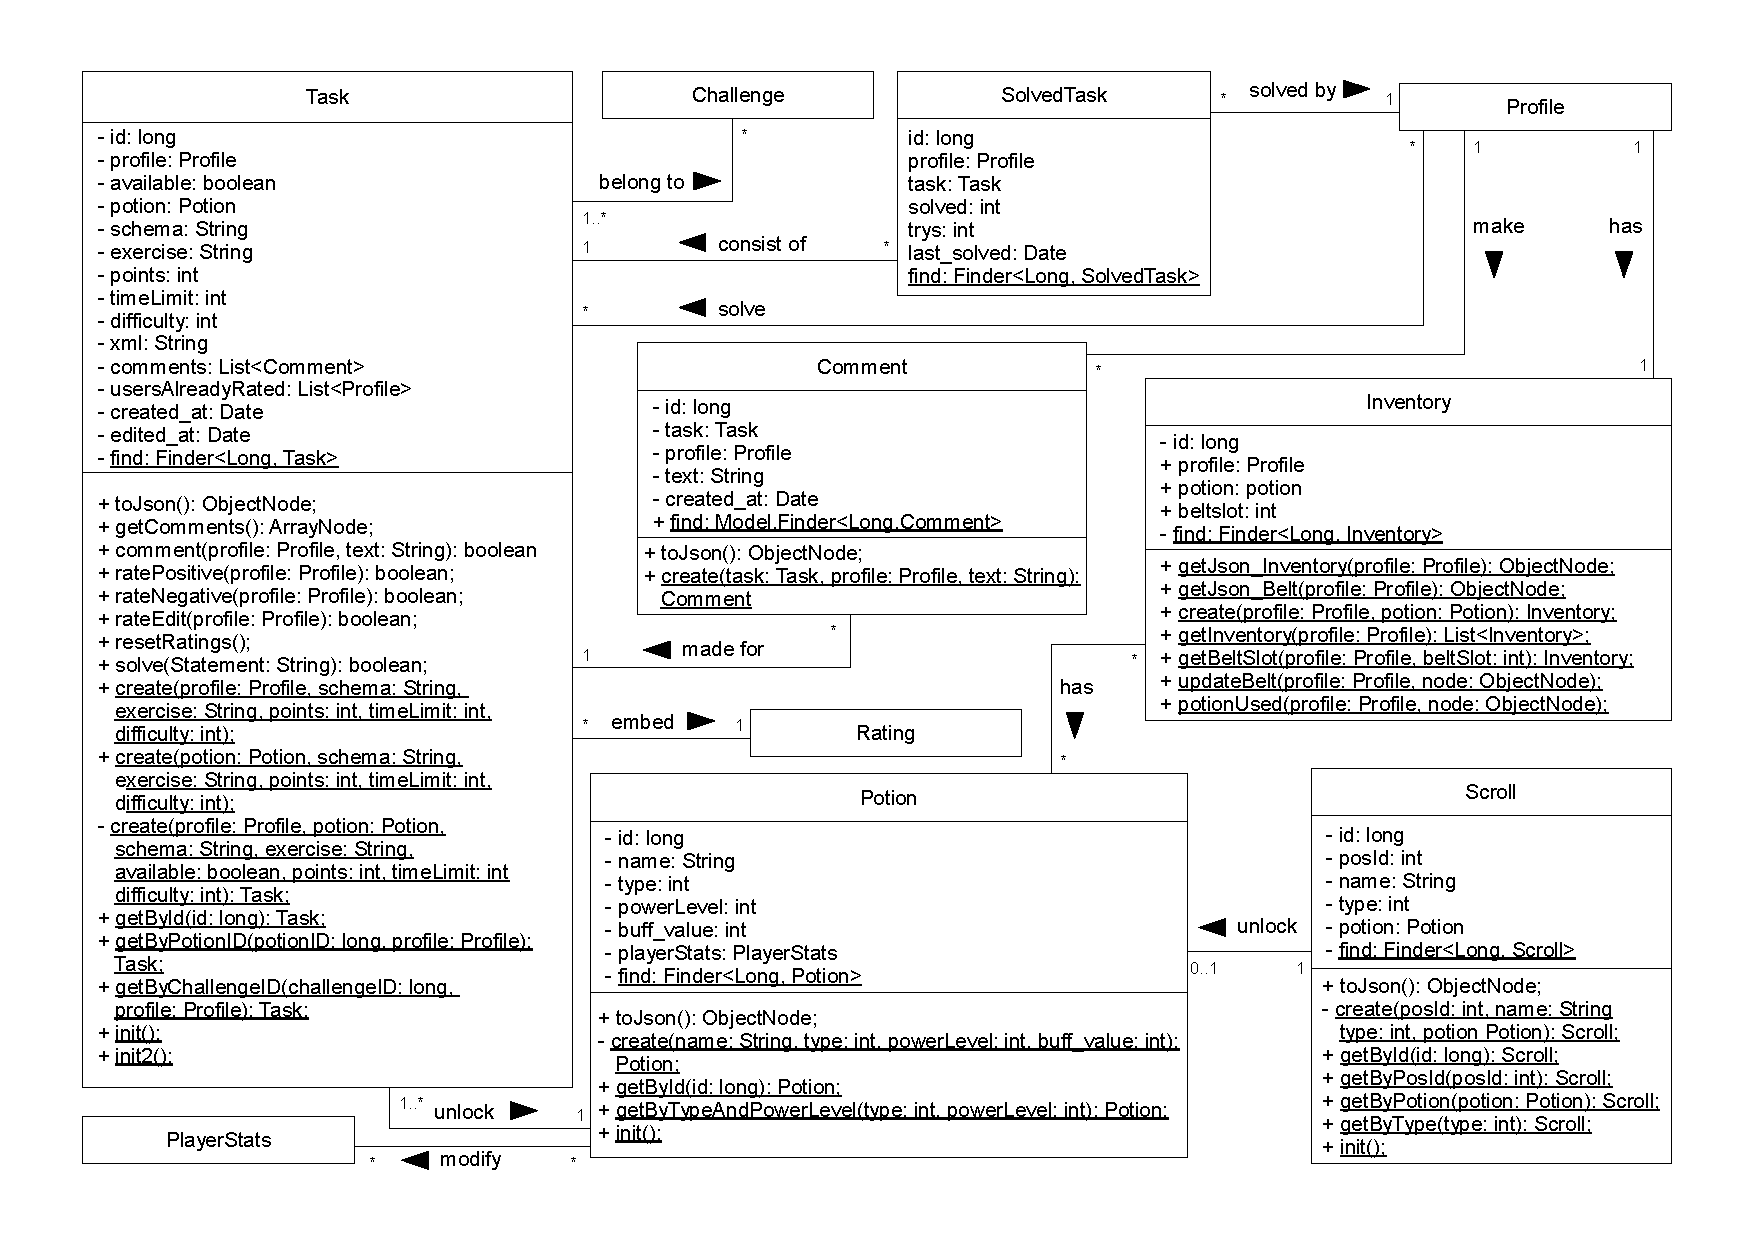
\includegraphics[width=0.8\textwidth]{figures/KDTaskAndInventory}
\caption{Klassendiagramm für einige der Model-Klassen \ref{C20}}
\label{classC10}
\end{figure}
\clearpage
\subsection{Erläuterung}
\begin{class}{120}{Task}
\item[Aufgabe]~\\
Verwaltung der Aufgaben inkl. Erstellung und Bewertung
\item[Attribute]~\\
\begin{itemize}
\item id: long -- Identität zur eindeutigen Identifizierung der Aufgabe
\item profile: Profile -- Profil, das der Aufgabe zugeordnet ist
\item available: boolean -- Verfügbarkeit der Aufgabe für den User
\item potion: Potion -- Trank, den der Spieler durch die erfolgreiche Bearbeitung der Aufgabe erhält
\item schema: String -- Verwendetes Datenbankschema
\item exercise: String -- Aufgabenstellung
\item points: int -- Punkte der Aufgabe
\item timeLimit: int -- Zeitlimit der Aufgabe
\item difficulty: int -- Schwierigkeit der Aufgabe
\item xml: String -- XML-Datei, die die Aufgabe enthält
\item comments: List<Comment> -- Liste mit Kommentaren, die Nutzer für diese Aufgabe abgegeben haben
\item usersAlreadyRated: List<Profile> -- Liste mit den Profilen der Nutzer, die diese Aufgabe bereits bewertet haben
\item created\_at: Date -- Erstellungsdatum
\item edited\_at: Date -- Datum der letzten Bearbeitung
\item find: Finder<Long, Task> -- Finder zum Suchen von Objekten in der Datenbank
\end{itemize}
\item[Operationen]~\\
\begin{itemize}
\item toJson(): ObjectNode -- Erzeugung und Rückgabe der Aufgabe als Json-Objekt
\item getComments(): ArrayNode -- Rückgabe der Kommentare als JsonNode-Objekte
\item comment(profile: Profile, text: String): boolean -- Bewerten einer Aufgabe. Das Profil sowie der Kommentar als string werden übergeben
\item ratePositive(profile: Profile): boolean -- Aufgabe positiv bewerten
\item rateNegative(profile: Profile): boolean -- Aufgabe negativ bewerten
\item rateEdit(profile: Profile): boolean -- Aufgabe zur Nachbearbeitung markieren
\item resetRatings() -- Zurücksetzen der Bewertungen
\item solve(Statement: String): boolean -- Aufgabe lösen
\item create(profile: Profile, schema: String, exercise: String, points: int, timeLimit: int, difficulty: int) -- Aufgabe erstellen
\item create(potion: Potion, schema: String, exercise: String, points: int, timeLimit: int, difficulty: int) -- Aufgabe erstellen
\item create(profile: Profile, potion: Potion, schema: String, exercise: String, available: boolean, points: int, timeLimit: int difficulty: int): Task -- Aufgabe erstellen
\item getById(id: long): Task -- Rückgabe der Aufgabe der entsprechenden Identität
\item getByPotionID(potionID: long, profile: Profile): Task -- Rückgabe der Aufgabe anhand des Tranks
\item getByChallengeID(challengeID: long,  profile: Profile): Task -- Rückgabe der Aufgabe anhand der ChallengeID
\item init() -- Initiierung der Aufgaben
\item init2() -- Initiierung der Aufgaben
\end{itemize}
\item[Kommunikationspartner]~\\
\begin{itemize}
\item SolvedTask
\item Comment
\item Challenge
\item Rating
\item Potion
\item Profile
\end{itemize}
\end{class}

\newpage
\begin{class}{130}{SolvedTask}
\item[Aufgabe]~\\
Verwaltung der gelösten Aufgaben
\item[Attribute]~\\
\begin{itemize}
\item id: long -- Identität zur eindeutigen Identifizierung des Objekts
\item profile: Profile -- Profil des Users, der die Aufgabe gelöst hat
\item task: Task -- Verweis auf die Aufgabe
\item solved: int -- Anzahl, wie oft der User diese Aufgabe bereits gelöst hat
\item trys: int -- Anzahl der Versuche, die nötig waren, die Aufgabe zu lösen
\item last\_solved: Date -- Datum des letzten richtigen Lösens der Aufgabe
\item find: Finder<Long, SolvedTask> -- Finder zum Suchen von Objekten in der Datenbank
\end{itemize}
\item[Operationen]~\\
Keine
\item[Kommunikationspartner]~\\
\begin{itemize}
\item Task
\item Profile
\end{itemize}
\end{class}

\newpage
\begin{class}{140}{Comment}
\item[Aufgabe]~\\
Verwaltung der Kommentare zu den Aufgaben
\item[Attribute]~\\
\begin{itemize}
\item id: long -- Identität zur eindeutigen Identifizierung des Objekts
\item task: Task -- Die zum Kommentar zugehörige Aufgabe
\item profile: Profile -- Profil des Users, der die Bewertung abgegeben hat
\item text: String -- Kommentarinhalt
\item created\_at: Date -- Erstellungsdatum des Kommentars
\item find: Finder<Long, Comment> -- Finder zum Suchen von Objekten in der Datenbank
\end{itemize}
\item[Operationen]~\\
\begin{itemize}
\item toJson(): ObjectNode -- Rückgabe des Objekts als JsonNode
\item create(task: Task, profile: Profile, text: String):
   Comment -- Erstellung eines Kommentars
\end{itemize}
\item[Kommunikationspartner]~\\
\begin{itemize}
\item Task
\item Profile
\end{itemize}
\end{class}

\newpage
\begin{class}{150}{Potion}
\item[Aufgabe]~\\
Verwaltung der Tränke
\item[Attribute]~\\
\begin{itemize}
\item id: long -- Identität zur eindeutigen Identifizierung des Objekts
\item name: String -- Name des Tranks
\item type: int -- Art des Tranks
\item powerLevel: int -- Stärke des Tranks
\item buff\_value: int -- Wert, um den das entsprechende Attribut verändert wird
\item playerStats: PlayerStats -- Objekt mit den Eigenschaften des Avatars
\item find: Finder<Long, Potion> -- Finder zum Suchen von Objekten in der Datenbank
\end{itemize}
\item[Operationen]~\\
\begin{itemize}
\item toJson(): ObjectNode -- Rückgabe des Objekts als JsonNode
\item create(name: String, type: int, powerLevel: int, buff\_value: int): Potion -- Erstellen neuer Tränke
\item getById(id: long): Potion -- Rückgabe eines Tranks anhand der ID
\item getByTypeAndPowerLevel(type: int, powerLevel: int): Potion -- Rückgabe des Tranks anhand des Typs und des PowerLevels
\item init() -- Initiierung der Tränke
\end{itemize}
\item[Kommunikationspartner]~\\
\begin{itemize}
\item Task
\item PlayerStats
\item Scroll
\item Inventory
\end{itemize}
\end{class}

\newpage
\begin{class}{160}{Inventory}
\item[Aufgabe]~\\
Inventar des Spielers
\item[Attribute]~\\
\begin{itemize}
\item id: long -- Identität zur eindeutigen Identifizierung des Objekts
\item profile: Profile -- Profil des Users
\item potion: potion -- Trank des Users
\item beltslot: int -- Gürtelslot
\item find: Finder<Long, Inventory> -- Finder zum Suchen von Objekten in der Datenbank
\end{itemize}
\item[Operationen]~\\
\begin{itemize}
\item getJson\_Inventory(profile: Profile): ObjectNode -- Rückgabe des Inventars als JSonNode-Objekt
\item getJson\_Belt(profile: Profile): ObjectNode -- Rückgabe des Gürtels als JSonNode-Objekt
\item create(profile: Profile, potion: Potion): Inventory -- Trank dem Inventar hinzufügen
\item getInventory(profile: Profile): List<Inventory> -- Rückgabe der Inventare
\item getBeltSlot(profile: Profile, beltSlot: int): Inventory -- Rückgabe des Gürtelslots
\item updateBelt(profile: Profile, node: ObjectNode) -- Update des Gürtels
\item potionUsed(profile: Profile, node: ObjectNode) -- Benutzte Tränke aus dem Inventar löschen
\end{itemize}
\item[Kommunikationspartner]~\\
\begin{itemize}
\item Task
\item PlayerStats
\item Scroll
\end{itemize}
\end{class}

\newpage
\begin{class}{170}{Scroll}
\item[Aufgabe]~\\
Verwaltung der im Spiel verwendeten Schriftrollen
\item[Attribute]~\\
\begin{itemize}
\item id: long -- Identität zur eindeutigen Identifizierung des Objekts
\item posId: int -- Positions-ID
\item name: String -- Name der Schriftrolle
\item type: int -- Art der Schriftrolle
\item potion: Potion -- Angabe des Tranks, der durch die Schriftrolle freigeschaltet werden kann
\item find: Finder<Long, Scroll> -- Finder zum Suchen von Objekten in der Datenbank
\end{itemize}
\item[Operationen]~\\
\begin{itemize}
\item toJson(): ObjectNode -- Rückgabe der Schriftrolle als Json-Objekt
\item create(posId: int, name: String
   type: int, potion Potion): Scroll -- Schriftrolle erstellen
\item getById(id: long): Scroll -- Rückgabe der Schriftrolle mit der entsprechenden ID
\item getByPosId(posId: int): Scroll -- Rückgabe der Schriftrolle entsprechend der Positions-ID im Spiel
\item getByPotion(potion: Potion): Scroll -- Rückgabe der Schriftrolle entsprechend des freischaltbaren Tranks
\item getByType(type: int): Scroll -- Rückgabe der Schriftrolle entsprechend des Typs
\item init() -- Initiierung der Schriftrollen
\end{itemize}
\item[Kommunikationspartner]~\\
\begin{itemize}
\item Potion
\end{itemize}
\end{class}

\newpage
\subsection{Helper and Secured Classes}
\subsection{Paket-/Klassendiagramm}
\begin{figure}[h!]
\centering
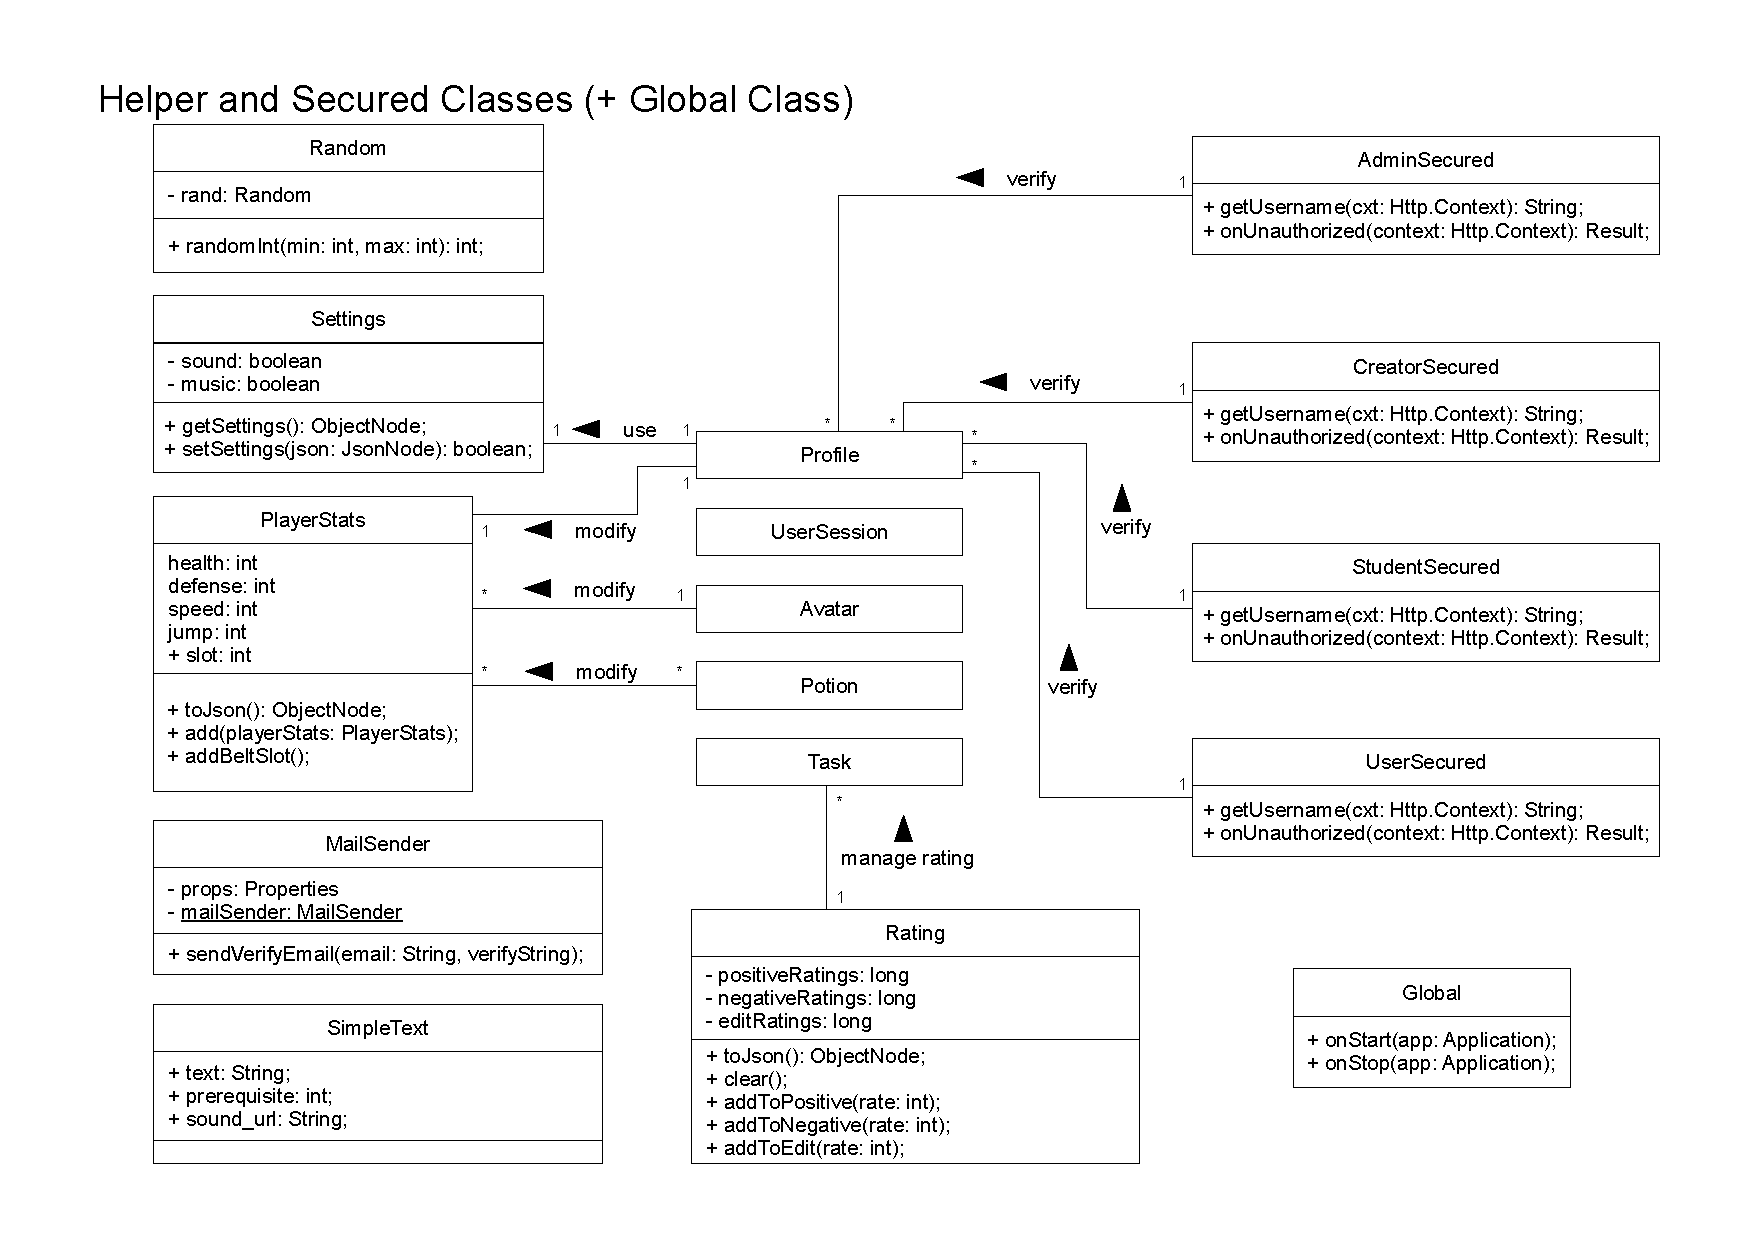
\includegraphics[width=0.8\textwidth]{figures/KDHelper}
\caption{Klassendiagramm für die Helper- und Secured-Klassen \ref{C20}}
\label{classC10}
\end{figure}
\clearpage
\subsection{Erläuterung}
\begin{class}{180}{Random}
\item[Aufgabe]~\\
Generierung von Zufallszahlen
\item[Attribute]~\\
\begin{itemize}
\item rand: Random -- Instanz der Klasse java.util.Random()
\end{itemize}
\item[Operationen]~\\
\begin{itemize}
\item randomInt(min: int, max: int): int -- Generierung einer Zufallszahl im angegebenen offenen Intervall
\end{itemize}
\item[Kommunikationspartner]~\\
Keine
\end{class}

\newpage
\begin{class}{190}{Settings}
\item[Aufgabe]~\\
Verwaltung der Benutzereinstellungen
\item[Attribute]~\\
\begin{itemize}
\item sound: boolean -- Soundeffekte sind entweder ein- oder ausgeschaltet
\item music: boolean -- Hintergrundmusik ist entweder ein- oder ausgeschaltet
\end{itemize}
\item[Operationen]~\\
\begin{itemize}
\item getSettings(): ObjectNode -- Rückgabe der Einstellungen als Json-Objekt
\item setSettings(json: JsonNode): boolean -- Einstellungen setzen
\end{itemize}
\item[Kommunikationspartner]~\\
\begin{itemize}
\item Profile
\end{itemize}
\end{class}

\newpage
\begin{class}{200}{PlayerStats}
\item[Aufgabe]~\\
Statistiken des Spielers
\item[Attribute]~\\
\begin{itemize}
\item health: int -- Gesundheit
\item defense: int -- Verteidigung
\item  speed: int -- Geschwindigkeit
\item jump: int -- Sprungkraft
\item  slot: int -- Anzahl der Taschenslots
\end{itemize}
\item[Operationen]~\\
\begin{itemize}
\item toJson(): ObjectNode -- Rückgabe der Statistik als Json-Objekt
\item add(playerStats: PlayerStats) -- Hinzufügen der Statistik
\item addBeltSlot() -- Taschenslot hinzufügen
\end{itemize}
\item[Kommunikationspartner]~\\
\begin{itemize}
\item Profile
\item Avatar
\item Potion
\end{itemize}
\end{class}

\newpage
\begin{class}{210}{MailSender}
\item[Aufgabe]~\\
Versenden von Emails
\item[Attribute]~\\
\begin{itemize}
\item props: Properties -- Properties-Objekt mit den Einstellungen
\item mailSender: MailSender -- Instanz der Klasse für die gesamte Anwendung
\end{itemize}
\item[Operationen]~\\
\begin{itemize}
\item sendVerifyEmail(email: String, verifyString) -- Versenden der Verifizierungsnachricht
\end{itemize}
\item[Kommunikationspartner]~\\
Keine
\end{class}

\newpage
\begin{class}{220}{SimpleText}
\item[Aufgabe]~\\
Verwaltung der Texte
\item[Attribute]~\\
\begin{itemize}
\item text: String -- Text
\item prerequisite: int -- Voraussetzung
\item sound\_url: String -- Referenz auf den Sound
\end{itemize}
\item[Operationen]~\\
Keine
\item[Kommunikationspartner]~\\
Keine
\end{class}

\newpage
\begin{class}{230}{Rating}
\item[Aufgabe]~\\
Bewertung der Aufgaben
\item[Attribute]~\\
\begin{itemize}
\item positiveRatings: long -- Anzahl der positiven Bewertungen
\item negativeRatings: long -- Anzahl der negativen Bewertungen
\item editRatings: long -- Anzahl, wie oft die Aufgabe zur Nachbearbeitung empfohlen wurde
\end{itemize}
\item[Operationen]~\\
\begin{itemize}
\item toJson(): ObjectNode -- Rückgabe als Json-Objekt
\item clear() -- Bewertung zurücksetzen
\item addToPositive(rate: int) -- Positive Bewertung hinzufügen
\item addToNegative(rate: int) -- Negative Bewertung hinzufügen
\item addToEdit(rate: int) -- Anzahl der Nutzer, die die Aufgabe zur Überarbeitung empfohlen haben
\end{itemize}
\item[Kommunikationspartner]~\\
\begin{itemize}
\item Task
\end{itemize}
\end{class}

\newpage
\begin{class}{240}{AdminSecured}
\item[Aufgabe]~\\
Berechtigung für Admintool
\item[Attribute]~\\
Keine
\item[Operationen]~\\
\begin{itemize}
\item getUsername(cxt: Http.Context): String -- Rückgabe des Benutzernamens
\item onUnauthorized(context: Http.Context): Result -- Result-Objekt mit einer Fehlermeldung bei unberechtigem Zugriff
\end{itemize}
\item[Kommunikationspartner]~\\
\begin{itemize}
\item UserSession
\end{itemize}
\end{class}

\newpage
\begin{class}{250}{CreatorSecured}
\item[Aufgabe]~\\
Berechtigung geschützten Bereich
\item[Attribute]~\\
Keine
\item[Operationen]~\\
\begin{itemize}
\item getUsername(cxt: Http.Context): String -- Rückgabe des Benutzernamens
\item onUnauthorized(context: Http.Context): Result -- Result-Objekt mit einer Fehlermeldung bei unberechtigem Zugriff
\end{itemize}
\item[Kommunikationspartner]~\\
\begin{itemize}
\item UserSession
\end{itemize}
\end{class}

\newpage
\begin{class}{260}{StudentSecured}
\item[Aufgabe]~\\
Berechtigung geschützten Bereich
\item[Attribute]~\\
Keine
\item[Operationen]~\\
\begin{itemize}
\item getUsername(cxt: Http.Context): String -- Rückgabe des Benutzernamens
\item onUnauthorized(context: Http.Context): Result -- Result-Objekt mit einer Fehlermeldung bei unberechtigem Zugriff
\end{itemize}
\item[Kommunikationspartner]~\\
\begin{itemize}
\item UserSession
\end{itemize}
\end{class}

\newpage
\begin{class}{270}{UserSecured}
\item[Aufgabe]~\\
Berechtigung geschützten Bereich
\item[Attribute]~\\
Keine
\item[Operationen]~\\
\begin{itemize}
\item getUsername(cxt: Http.Context): String -- Rückgabe des Benutzernamens
\item onUnauthorized(context: Http.Context): Result -- Result-Objekt mit einer Fehlermeldung bei unberechtigem Zugriff
\end{itemize}
\item[Kommunikationspartner]~\\
\begin{itemize}
\item UserSession
\end{itemize}
\end{class}

\newpage
\begin{class}{280}{Global}
\item[Aufgabe]~\\
Verwaltung der Methoden zum Starten und Beenden
\item[Attribute]~\\
Keine
\item[Operationen]~\\
\begin{itemize}
\item onStart(app: Application) -- Aufruf beim Starten
\item onStop(app: Application) -- Aufruf beim Beenden
\end{itemize}
\item[Kommunikationspartner]~\\
Keine
\end{class}

\newpage
\begin{class}{290}{Application}
\item[Aufgabe]~\\
Die Methoden dieser Klasse liefern die Content-Seiten mit einem Authorisierungsschlüssel an den Benutzer. Der Schlüssel legt dabei die Berechtigungen fest
\item[Attribute]~\\
Keine
\item[Operationen]~\\
\begin{itemize}
\item admin(): Result -- Rückgabe eines Result-Objekts mit dem Inhalt "Admin"
\item init(): Result -- Initiierungsmethode
\end{itemize}
\item[Kommunikationspartner]~\\
\begin{itemize}
\item All model classes
\end{itemize}
\end{class}

\newpage
\subsection{Controller Classes}
\subsection{Paket-/Klassendiagramm}
\begin{figure}[h!]
\centering
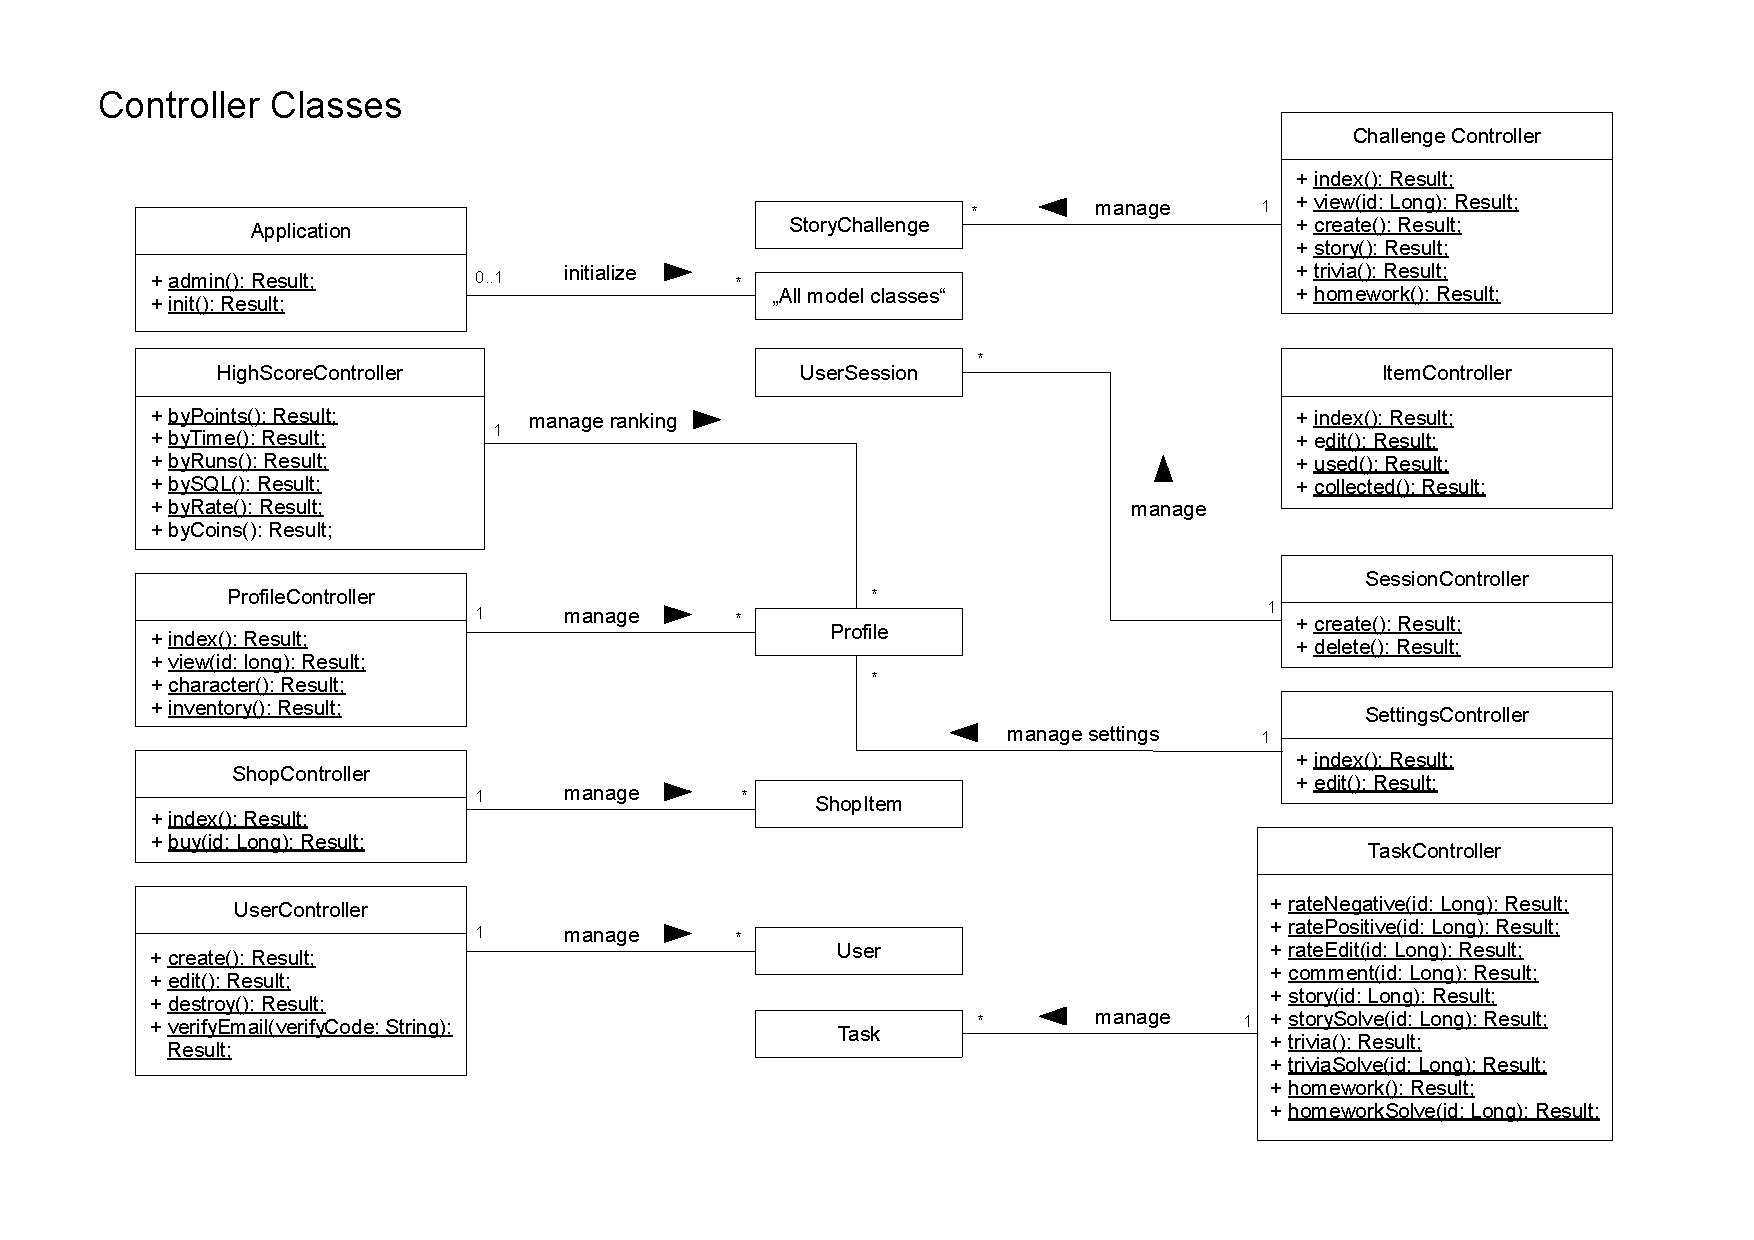
\includegraphics[width=0.8\textwidth]{figures/KDController}
\caption{Klassendiagramm für die Controller-Klassen \ref{C20}}
\label{classC10}
\end{figure}
\clearpage
\subsection{Erläuterung}
\begin{class}{300}{HighScoreController}
\item[Aufgabe]~\\
Methoden zur Sortierung der HighScore-Listen
\item[Attribute]~\\
Keine
\item[Operationen]~\\
\begin{itemize}
\item byPoints(): Result -- Sortierung nach Punkten
\item byTime(): Result -- Sortierung nach Zeit
\item byRuns(): Result -- Sortierung nach Runs
\item bySQL(): Result -- Sortierung nach gelösten SQL-Aufgaben
\item byRate(): Result -- Sortierung nach Bewertung
\item byCoins(): Result -- Sortierung nach Münzen
\end{itemize}
\item[Kommunikationspartner]~\\
\begin{itemize}
\item Profile
\end{itemize}
\end{class}

\newpage
\begin{class}{310}{ProfileController}
\item[Aufgabe]~\\
Methoden zur Benutzung der Profile
\item[Attribute]~\\
Keine
\item[Operationen]~\\
\begin{itemize}
\item index(): Result -- Rückgabe der Spielstatistik als Json-Objekt
\item view(id: long): Result -- Rückgabe des Profils entsprechend der ID
\item character(): Result -- Rückgabe des Charakterzustands als Json-Objekt
\item inventory(): Result -- Rückgabe des Inventars
\end{itemize}
\item[Kommunikationspartner]~\\
\begin{itemize}
\item Profile
\end{itemize}
\end{class}

\newpage
\begin{class}{320}{ShopController}
\item[Aufgabe]~\\
Methoden zur Benutzung der Objekte aus dem Shop
\item[Attribute]~\\
Keine
\item[Operationen]~\\
\begin{itemize}
\item index(): Result -- Rückgabe aller Shop-Gegenstände als Result-Objekt
\item buy(id: Long): Result -- Kauf eines Gegenstands
\end{itemize}
\item[Kommunikationspartner]~\\
\begin{itemize}
\item ShopItem
\end{itemize}
\end{class}

\newpage
\begin{class}{330}{UserController}
\item[Aufgabe]~\\
Methoden zur Benutzung des Benutzerobjekts
\item[Attribute]~\\
Keine
\item[Operationen]~\\
\begin{itemize}
\item create(): Result -- Erstellen eines Benutzerobjekts
\item edit(): Result -- Ändern des Passworts
\item destroy(): Result -- Löschen des Benutzerobjekts 
\item verifyEmail(verifyCode: String) -- Emailverifizierung
   Result;
\end{itemize}
\item[Kommunikationspartner]~\\
\begin{itemize}
\item User
\end{itemize}
\end{class}

\newpage
\begin{class}{340}{ChallengeController}
\item[Aufgabe]~\\
Methoden zur Benutzung des Herausforderungsobjekts
\item[Attribute]~\\
Keine
\item[Operationen]~\\
\begin{itemize}
\item index(): Result -- Rückgabe der Herausforderungen
\item view(id: Long): Result -- Ansicht der Herausforderung
\item create(): Result -- Erstellen der Herausforderung
\item story(): Result -- Herausforderung dem Profil zuordnen
\item trivia(): Result -- Rückgabe einer Triviaaufgabe
\item homework(): Result -- Rückgabe einer Hausaufgabe
\end{itemize}
\item[Kommunikationspartner]~\\
\begin{itemize}
\item StoryChallenge
\end{itemize}
\end{class}

\newpage
\begin{class}{350}{ItemController}
\item[Aufgabe]~\\
Methoden zur Benutzung der Gegenstände
\item[Attribute]~\\
Keine
\item[Operationen]~\\
\begin{itemize}
\item index(): Result -- Rückgabe der Gegenstände
\item edit(): Result -- Gegenstand bearbeiten
\item used(): Result -- Gegenstand benutzt
\item collected(): Result -- Gegenstand aufgesammelt
\end{itemize}
\item[Kommunikationspartner]~\\
\end{class}

\newpage
\begin{class}{360}{SessionController}
\item[Aufgabe]~\\
Methoden zur Verwaltung der aktuellen Sitzung
\item[Attribute]~\\
Keine
\item[Operationen]~\\
\begin{itemize}
\item create(): Result -- Sitzung erstellen
\item delete(): Result -- Sitzung löschen
\end{itemize}
\item[Kommunikationspartner]~\\
\begin{itemize}
\item UserSession
\end{itemize}
\end{class}

\newpage
\begin{class}{370}{SettingsController}
\item[Aufgabe]~\\
Methoden zur Verwaltung der aktuellen Einstellungen
\item[Attribute]~\\
Keine
\item[Operationen]~\\
\begin{itemize}
\item index(): Result -- Rückgabe der Einstellungen
\item edit(): Result -- neue Einstellungen übernehmen
\end{itemize}
\item[Kommunikationspartner]~\\
\begin{itemize}
\item Profile
\end{itemize}
\end{class}

\newpage
\begin{class}{380}{TaskController}
\item[Aufgabe]~\\
Methoden zur Verwaltung der aktuellen Aufgabe
\item[Attribute]~\\
Keine
\item[Operationen]~\\
\begin{itemize}
\item rateNegative(id: Long): Result -- Aufgabe positiv bewerten
\item ratePositive(id: Long): Result -- Aufgabe negativ bewerten
\item rateEdit(id: Long): Result -- Aufgabe zur Nachbearbeitung markieren
\item comment(id: Long): Result -- Aufgabe kommentieren
\item story(id: Long): Result -- Aufruf der Aufgabe aus dem Story-Modus
\item storySolve(id: Long): Result -- Lösen der Aufgabe
\item trivia(): Result -- Aufruf der Trivia-Aufgabe
\item triviaSolve(id: Long): Result -- Lösen einer Trivia-Aufgabe
\item homework(): Result -- Aufruf der Hausaufgabe
\item homeworkSolve(id: Long): Result -- Lösen der Hausaufgabe
\end{itemize}
\item[Kommunikationspartner]~\\
\begin{itemize}
\item Task
\end{itemize}
\end{class}
